\documentclass[a4paper,11pt,oneside,oldfontcommands]{memoir}
\usepackage{ecis2015}
\usepackage{datetime}    			% sourced from; http://ftp.snt.utwente.nl/pub/software/tex/macros/latex/contrib/datetime/
\usepackage{longtable}

%\usepackage{amssymb, setspace, rotating, titlesec, adjustbox, array, threeparttable}
\usepackage{amssymb, setspace, rotating, titlesec, adjustbox, array, threeparttable}
									% is all of this necessary?? 
%%%%%%%%%%%%%%%%%									
%% Fonts, fonts, fonts, notably for math
\usepackage{xfrac}					% tbv slanted fractions: \sfrac{}{}
\usepackage{pifont}

\RequirePackage[utf8]{inputenc}		% NOT required when using xetex as opposed to pdftex

\usepackage[T1]{fontenc}

\usepackage{amsmath}				% <amsmath> needs to be loaded before ntheorem (section 3.2.1, ftp://ftp.dante.de/pub/tex/macros/latex/contrib/ntheorem/ntheorem.pdf) 
\usepackage[mathcal]{euscript}		% tbv de gecalligrafeerde mathcal{O} en W(orld) en (M)odel etc. Refer to http://texdoc.net/texmf-dist/doc/fonts/amsfonts/euscript.pdf
									% Note that, in fact, eucal and euscript are identical, except that they use different commands (\mathcal and \mathscr). By using euscript 
									% we only provide \mathscr{} and leave \mathcal{} from amsmath unchanged
\usepackage{pgothic}				% Used for modern gothic that has a readible S
\DeclareMathAlphabet{\mathgoth}{T1}{pgoth}{m}{n}	% Declaring the pgothic family as math alphabet
%\usepackage{addfont}				% This would be an alternative for the readible S font, but not working
%\addfont[1.25]{OT1}{hge}{\hge}
%\DeclareMathAlphabet{\mathgoth}{OT1}{hge}{m}{n}	% Declaring the hge family as math alphabet

\usepackage{lmodern}				% necessary in combination with CMcal-font from mathcal/euscript to generate the font that is necessary for the Interpretation function \CMcal{I}
\usepackage{amssymb}				% necessary for (at least) the \mathbb font
\usepackage{mathrsfs}				% necessary for (at least) the \mathpzc font
\DeclareMathAlphabet{\mathpzc}{OT1}{pzc}{l}{it}		% Declaring the pzc font as math alphabet (not used, yet)


\usepackage[normalem]{ulem}			% tbv strikout text: \sout{deze tekst is strikeout}
\usepackage{siunitx}				% Necessary??

%\usepackage{fourier} 				% Assuming that you are using venturis for text, Hirwen Harendal, who designed the collection, advises that the best choice for mathematics is
									%	fourier and the second best is mathdesign. Fourier sets text and math fonts.
\usepackage{venturis2}				% Ik wil het font Venturis ADF No2 toepassen als Normalfont
									% 	Ik kan ook overwegen Obyknovennaya Novaya te gebruiken, ook fraai. Gevonden op http://www.tug.dk/FontCatalogue/venturisadfno2/

%% End of Fonts
%%%%%%%%%%%%%%%

\usepackage{xcolor}
%%\usepackage{MnSymbol}				% Levert foutmelding: Too many math alphabets used in version normal. 
\usepackage[xindy,toc]{glossaries}	%%%% The glossaries environment. Refer to: http://en.wikibooks.org/wiki/LaTeX/Glossary
%%%\usepackage{pst-plot}				%%%% The ps trick environment. Zie ook: http://tug.org/PSTricks/main.cgi?file=examples REQUIRES --latex-engine=xelatex

%% Theorems
\usepackage[ntheorem]{empheq}
\usepackage[thmmarks]{ntheorem}		% Easier handling of theorem-like environments. refer to ftp://ftp.dante.de/pub/tex/macros/latex/contrib/ntheorem/ntheorem.pdf

\usepackage{datetime}    			 % sourced from; http://ftp.snt.utwente.nl/pub/software/tex/macros/latex/contrib/datetime/
\usepackage{mdframed}

%% Figures and table placement		% Sourced from http://tug.ctan.org/tex-archive/info/epslatex/english/epslatex.pdf page 55
\usepackage{flafter}				% Ensure that the figures/tables appear after its figure/table environment definition in the text

\makeatletter						% Change the default figure / table placement from [tbp] to [htbp]; this is useful since mmd prevents us to insert the placement parameters ourselves
\def\fps@figure{htbp}
\def\fps@table{htbp}
\makeatother

\usepackage[section]{placeins}		% Since it is often desirable to keep floats in the section in which they were issued, insert a \FloatBarrier command before each section.

%% Drawings by LaTeXDraw
%\usepackage{auto-pst-pdf}			% To use pstricks in pdflatex: https://tex.stackexchange.com/questions/8413/how-to-use-pstricks-in-pdflatex
%\usepackage[pdf,usenames,dvipsnames]{pstricks}
%\usepackage{epsfig}
%\usepackage{pst-grad} % For gradients
% \usepackage{pst-plot} % For axes
%\usepackage[space]{grffile} % For spaces in paths
%\usepackage{etoolbox} % For spaces in paths
%\makeatletter % For spaces in paths
%\patchcmd\Gread@eps{\@inputcheck#1 }{\@inputcheck"#1"\relax}{}{}
%\makeatother


%% Logical proofs
\usepackage{lplfitch}				% sourced from https://github.com/rzach/lplfitch
%									% documentation from http://ftp.snt.utwente.nl/pub/software/tex/macros/latex/contrib/lplfitch/lplfitch.pdf
%\usepackage{fitch}					% The fitch package is more simple to use than lplfitch

%% Lists
%\usepackage[ampersand]{easylist}	% The easylist environment
\usepackage{enumitem}				% List manipulation package

%% Grammars
\usepackage[epsilon]{backnaur}		% For creation of BNF grammars. Refer to http://ctan.cs.uu.nl/macros/latex/contrib/backnaur/backnaur.pdf 

%% Lorem ipsum generated text
\usepackage{blindtext}

%% ToDo's							% Creating proper todo bubbles adjacent to text. Refer to http://ctan.triasinformatica.nl/macros/latex/contrib/todonotes/todonotes.pdf
\usepackage[textsize=tiny,colorinlistoftodos]{todonotes}	

%% Cross-referencing				% Allow the format of cross-references to be determined automatically according to the “type” of cross-reference (equation, section, etc.) and the context in which the cross-reference is used.
%\usepackage{varioref}				% sourced from http://texdoc.net/texmf-dist/doc/latex/tools/varioref.pdf
\usepackage{hyperref}				% If we want to use hyperref, sometime in the future for some reason, it should be defined in between of varioref and cleveref
\usepackage{cleveref}				% sourced from http://tug.ctan.org/macros/latex/contrib/cleveref/cleveref.pdf Makes varioref clever, and reuses its work to improve its own workings. 
									% The cleveref package must be loaded after all other packages that don’t specifically support it.
									% Therefore, to be safe, we declare it as last in the document's preamble.
									% Also note that all \newtheorem definitions must be placed after the cleveref package is loaded.

%% Table stuff						% sourced from: https://tex.stackexchange.com/questions/33510/how-do-i-create-the-headings-for-this-multirow-multicolum-table
\usepackage{graphicx}
\usepackage{multirow}
\usepackage{booktabs}

%%% About this LaTeX template: %%%%%%%%%%%%%%%%%%%%%%%%%%%%%%%%%%%%%%%%%%%%%%%
%
% This template should work with any (reasonably recent) full
% installation of TeXLive or MikTeX. The "ecis2015" package loads a
% number of other packages, so if some package is missing, please
% install it using the package manager of your TeX distribution. In
% particular, if the "tikz" package is missing, you may have to install
% "pgf" or simply remove our example graphics (see figure example
% below).
%
% The file "ecis2015.sty" should be placed somewhere in your TeX Path
% (or simply in the same folder as your document).
%
% Please use PDFLaTeX to compile your document.
%
% You need not escape special characters or Umlauts like é ä ö ü ß (in 
% fact, you shouldn't), as this source is inputenc'd in UTF-8.
%
% Note for BibTeX users: We use BibLaTeX for formatting, so we use Biber
% as a sorting backend (default). 
% If you still need to use the old BibTeX program, please change the 
% BibLaTeX backend in the package file ("ecis2015.sty").
%
%%%%%%%%%%%%%%%%%%%%%%%%%%%%%%%%%%%%%%%%%%%%%%%%%%%%%%%%%%%%%%%%%%%%%%%%%%%%%%


%%% ------- mijn configs: --------- %%%
%
%% test stuff

% Redefining the paragraph level into a case - see https://tex.stackexchange.com/questions/129208/numbering-paragraphs-in-latex
\newcounter{para}
\renewcommand\paragraph[1]{%
  {\par\refstepcounter{para}\textbf{Case \thepara:\space#1\space}\label{#1}}
}

%% end test stuff


%%
%% Defining new theorem and -styles
% Its documentation can be found at ftp://ftp.dante.de/pub/tex/macros/latex/contrib/ntheorem/ntheorem.pdf
%\RequirePackage[thref, thmmarks, amsmath]{ntheorem}		% Use new theorems package as opposed to amsth, include <amsmath>-emulation by including it as an option

% Allow to repeat a theorem number to, e.g., continue with a theorem such as an example, or to add something to an existing theorem
% THIS UNFORTUNATELY DOES NOT WORK, producing a <Undefined control sequence \n <argument> \rep@title \n l.38 \newtheorem*{rep@theorem}{\rep@title}>-error
%\makeatletter
%\newtheorem*{rep@theorem}{\rep@title}
%\newcommand{\newreptheorem}[2]{%
%\newenvironment{rep#1}[1]{%
% \def\rep@title{#2 \ref{##1}}%
% \begin{rep@theorem}}%
% {\end{rep@theorem}}}
%\makeatother
	
%%%%% Theorems Definitions %%%%%%
\theoremstyle{definition}
\theoremstyle{break}		% The header for all theorems are followed by a newline
% Examples 					-- are numbered by chapter, and carry an asterisk as closing symbol
\theoremsymbol{\ensuremath{_\Box}}
\newtheorem{mmexmp}{Example}[chapter]
%\newreptheorem{mmexmp}{Example (cont'd)}
% Theses   					-- have continuous numbering scheme, and still close with the asterisk
\newtheorem{Thesis}{Thesis}
% Research Questions 		-- are enclosed with horizontal lines, and probably (?) close with the asterisk
\theoremprework{\hrule}
\theorempostwork{\hrule}
\newtheorem{mmthrq}{Research Question}
% Assumption				-- are numbered by chapter, and carry an asterisk as closing symbol
\newtheorem{mmasmptn}{Assumption}[chapter]
% Definitions & theorems	-- are numbered by chapter, and carry a black square as closing symbol
\theoremsymbol{\ensuremath{_\blacksquare}}
\newtheorem{mmdef}{Definition}[chapter]
\newtheorem{mmtrm}{Theorem}[chapter]
% Design Principles, proofs	-- are numbered by chapter, and carry an open diamond as closing symbol
\theoremsymbol{\ensuremath{_\diamond}}
\newtheorem{mmdp}{Design Principle}[chapter]
\newtheorem{mmprf}{Proof}[chapter]
% Remarks to tables, figures, whatever -- restart numbering at sections, no closing symbol
\theoremsymbol{}			% no symbol
\theorembodyfont{\upshape}	% no slanted or italics
\newtheorem{mmrmk}{Remark}[subsection]	% theorem counter resets every \subsection
\renewcommand{\themmrmk}{(\arabic{mmrmk})}	% Remove subsection from theorem counter representation

% Names of the theorems
\crefname{mmexmp}{Example}{Examples}
\crefname{Thesis}{Thesis}{Theses}
\crefname{mmthrq}{Research Question}{Research Questions}
\crefname{mmdef}{Definition}{Definitions}
\crefname{mmtrm}{Theorem}{Theorems}
\crefname{mmprf}{Proof}{Proofs}
\crefname{mmdp}{Design Principle}{Design Principles}
\crefname{mmasmptn}{Assumption}{Assumptions}
\crefname{mmrmk}{Remark}{Remarks}
\crefname{chapter}{Chapter}{Chapters}
\crefname{section}{Section}{Sections}
\crefname{figure}{Figure}{Figures}
\crefname{table}{Table}{Tables}
\crefname{equation}{Eq.}{Eqs.}

% Definition of List of Theorems (\listtheorems{<name>})
\theoremlisttype{opt}

%%%%%%%% End Theorems definitions

% Equations				-- are numbered by chapter
\numberwithin{equation}{chapter}
% Figures				-- are numbered by chapter
\numberwithin{figure}{chapter}

% package backnaur: modify the production operator
\renewcommand*{\bnfpo}{\textnormal{::=}}

% some more mnemonic terms 
\newcommand*\OK{\ding{51}}		% for the check-marks
\newcommand*\ntsa{\ensuremath{\varnothing}}	% no transcription allowed

% Create a typical column header, the content of which is rotated
\newcolumntype{R}[2]{%
 >{\adjustbox{angle=#1,lap=\width-(#2)}\bgroup}%
 l%
 <{\egroup}%
}
\newcommand*\rot{\multicolumn{1}{R{60}{1em}}}% no optional argument here, please!

% Create a command for words in a box. Refer to http://tex.stackexchange.com/questions/86569/creating-uniformly-sized-boxes-around-text, and 
%                                      for the colors to http://tex.stackexchange.com/questions/136742/changing-background-color-of-text-in-latex
\newcommand{\mywordbox}[1]{%
  {% open a group for a local setting
   \setlength{\fboxsep}{-2\fboxrule}% the rule will be inside the box boundary
   \hspace{1pt}\fcolorbox{gray!20}{blue!5}{\hspace{2pt}\strut\textbf{#1}\hspace{2pt}}\hspace{1pt}% print the box, with some padding at the left and right
%   \fbox{\hspace{2pt}\strut\text{#1}\hspace{2pt}}% print the box, with some padding at the left and right
%   \fbox{\hspace{2pt}\strut#1\hspace{2pt}}% print the box, with some padding at the left and right
  }% close the group
}


%%% Enter Document Info here: %%%%%%%%%%%%%%%%%%%%%%%%%%%%%%%%%%%%%%%%%%%%%%%%
%%%datetime package config %%%
\renewcommand{\dateseparator}{-}
%\renewcommand{\timeseparator}{}
\settimeformat{hhmmsstime}  

\maintitle{Consolidating semantic interoperability in contemporary architectural
paradigms} % ← Don't use UPPERCASE here, we do that automatically.
\subtitle{}
\shorttitle{} % ← This goes into the header.
\category{} % 
\versionmgt{version: v0.3-16}
\date{\today}


\authors{% Separate authors by a "\par" or blank line.
Paul Brandt,\\
Eindhoven University of Technology; Netherlands Organization of Applied
Scientific Research TNO, Den Haag, The Netherlands, 

\par
Eric Grandry,\\
Luxembourg Institute of Science and Technology, Esch-sur-Alzette,
Luxembourg, 

\par
Twan Basten,\\
Eindhoven University of Technology, Eindhoven, The Netherlands, 

\par
}
\shortauthors{Paul Brandt -- } % ← This goes into the header. 

%%% BibTeX: %%%%%%%%%%%%%%%%%%%%%%%%%%%%%%%%%%%%%%%%%%%%%%%%%%%%%%%%%%%%%%%%%%

\addbibresource{src/bib/CitedByMe-2018\_archSIOp.bib} % ← Your .bib file, if you're using BibTeX

%%%%%%%%%%%%%%%%%%%%%%%%%%%%%%%%%%%%%%%%%%%%%%%%%%%%%%%%%%%%%%%%%%%%%%%%%%%%%%

%%% Glossaries: %%%%%%%%%%%%%%%%%%%%%%%%%%%%%%%%%%%%%%%%%%%%%%%%%%%%%%%%%%%%%%

%%%%%%%%%%%%%%%%%%%%%%%%%%%%%%%%%%%%%%%%%%%%%%%%%%%%%%%%%%%%%%%%%%%%%%%%%%%%%%

\begin{document}
% Set the properties of the easylist

%\pagebreak

% --- Abstract --- --- --- --- ---
\begin{abstract}
\emph{Context:} Access-and-Play semantic interoperability (sIOP) is the
next glass ceiling in IT-based business collaboration. Current
approaches towards sIOP rely on conventions on the semantics of the
exchanged terms, which can be considered accepted folklore. Approaches
to break through the ceiling require some level of automation, and
artificial intelligence (AI) can make a difference.

\emph{Objective:} The objective of this study is to identify and define
AI-based fundamental guidance towards access-and-play sIOP in
contemporary architectural paradigms.

\emph{Method:} Our approach is based on the discipline of semiotics. We
identify semiotic shortcomings in architectures, establish a semiotic
explanation on software semantics and, subsequently, on sIOP. Based on
these considerations, we develop guiding architectural principles in
support of software semantics and sIOP. We evaluate these principles by
designing and formulating an ISO-42010 Architecture Viewpoint and View
on sIOP.

\emph{Results:} The semiotic approach demonstrates semantics in software
to be the result of a reciprocity between data and the software code
that operates on them. Data exchange breaks that reciprocity and the
main concern of sIOP is to re-establish a valid reciprocity. Loosely
coupled semantics, semantic alignments and an ontological commitment of
the modelling language can be considered the cornerstone to achieve
sIOP. The supporting principles are (i) semantic transparency, (ii)
semantic separation of concerns, and (iii) explicit computational
semantics. The resulting ISO-42010 Architecture Viewpoint and View on
sIOP, including a semantic mediation capability, can be considered a
pattern to consolidate sIOP in contemporary architectural paradigms.

\emph{Conclusions:} The major shortcomings in architectural paradigms to
account for sIOP are their negligence of semiotic fundamentals and the
absence of an explicit ontological commitment that stands at the root of
semantics. By their explicit inclusion, access-and-play sIOP can be
consolidated in contemporary architectural paradigms.\\
\end{abstract}


% --- Keywords --- --- --- --- ---



%\pagebreak
% --- table of contents --- --- --- --- ---
%
% add table of contents to pdf bookmarks


% add list of todo's that are outstanding for this text


% --- main matter --- --- --- --- ---

\hypertarget{introduction}{%
\chapter{Introduction}\label{introduction}}

Never before, data were so ubiquitous, and managed access to external
data was so easy. Because current ICT is unable to \emph{use} all that
same external, non-native data as access-and-play service, agility in
business collaboration is hampered in all domains. For instance,
consider the following (allegedly real) example of an interoperability
failure.{[} brandtp, 9/5/2018 We can apply another example, I'm open to
that. Indeed a TOOP example could be appropriate. However, I cannot
think of one but maybe Eric can?{]}

\begin{quote}
A German steel producer upgraded its industrial process robot. Since the
majority of the steel production process is dependent on time, from a
security point of view the decision was made to not rely on their own
internal clocks but to use the German \emph{Braunschweig Funkuhr} time
radio signal as source for the exact time instead. At the end of April
1993, when Germany went on summer time, the computer clock of the steel
producer went from 1:59 AM to 3:00 AM in one minute. This resulted in a
production line allowing molten ingots to cool for one hour less than
normal. When the process controller thought the cooling time had
expired, his actions splattered still-molten steel, damaging part of the
facility.\footnote{Source:
  http://catless.ncl.ac.uk/Risks/14.57.html\#subj1, accessed May 20,
  2018}
\end{quote}

In this simple example a tiny difference in the meaning of \texttt{time}
between the steel producer and the national time provider hampered
interoperability to the extend of damaging the steel facility. This tiny
difference rooted in the assumption by the steel producer that
\texttt{time} expressed a continuous scale whilst for the Braunschweig
Funkuhr, \texttt{time} denoted instant clock time for that time zone and
therefore represented a non-continuous scale. In order to achieve that
both collaborators, here the Braunschweig Funkuhr and the steel
producer, can actually \emph{use} their peers data, the need exists to
design and implement wrappers that remove any inconsistency between the
variations that may occur in terms, structures, dimensions and what have
you. Many such variations exist, leading to a range of failures in
so-called \emph{semantic interoperability} (sIOP) and Section/Appendix
\#\#{[} brandtp, 9/5/2018 Add sIOP-faults as appendix.{]} provides for a
short overview of sIOP-faults. Unfortunately, it is fundamentally
impossible to automate the production of wrappers, because we need a
genuine \emph{understanding} upfront, which computers still cannot do.

The most disconcerting consequences of a lack of (automated) sIOP are
time-to-deliver, flat interoperability failures, and even seemingly
correct but quite invalid data analysis probably leading to faulty
system behaviour. Current sIOP implementations are essentially based on
the (time-consuming) process of establishing a (local) convention on the
semantics of the terms that are exchanged during collaboration,
requiring custom solutions and collaboration-dependent software
adaptations. Such conventions can be considered a semantic monolith,
which makes dealing with data outside the monolith impossible, unless
again a time consuming (months) semantic adoption process is applied.
Moreover, these semantic conventions consider semantic heterogeneity as
a bug instead of a feature necessary to achieve semantic accuracy. But
still, this conventions-based approach towards sIOP is accepted folklore
in ICT. In view of the large uptake of the Internet, the Internet of
Things (IoT), cloud computing and big data, and in view of economical
pressure to intensify enterprise collaboration, we consider this
approach ``too little, too late''. Some form of automation is required
to resolve these issues, and we place artificial intelligence (AI) at
its core. With the separation (coined by Searle 1980) between
\emph{strong} AI (a system that can \emph{think} and has a \emph{mind},
in the philosophical definition of the term) or \emph{weak} AI (a system
that can only \emph{act} like it thinks and has a mind), we take the
position that --unfortunately-- strong AI is not yet available, if ever
(Xiuquan Li and Tao Zhang 2017). We therefore make do with weak AI and
show that despite its limitations it still has got a fundamental role to
fulfil as carrier for semantics and sIOP, both facilitating the required
automation. Weak AI, despite its current applications in Semantic Web or
ontologies, has not yet been embedded in contemporary software
architectural paradigms.

In comparison, scalability was a big architectural concern in the past,
requiring custom solutions as well. In response to this concern,
scalability was standardised in the form of architectural patterns, and
finally totally embedded and hidden into the infrastructure. Similarly,
sIOP can be considered the architectural concern of this decade. We
first need to provide a standardised solution pattern to address
semantic concerns before we can embed it in a technological
infrastructure. Only then we can claim that sIOP becomes transparent to
the developer and that the semantic monolith is taken down. Where
scalability resulted in a huge increase in performance-demanding
applications against a fraction of the original costs and effort,
business agility will emerge once the semantic monolith is removed and
semantic services exist at the infrastructural level. Then sIOP becomes
an access-and-play operation that can be achieved with data not
anticipated for during software design in due time, at any point in
their life cycle. Metaphorically speaking, we consider sIOP as a
\emph{bridge} overarching a (semantic) gap: with \emph{bridgeheads}
(semantic concerns) on each side of the gap, with a \emph{spanning}
(semantic aligments) resting on them to structurally support the bridge
and its traffic, and with a \emph{roadway} (data mediation) enabling the
crossing of the traffic. Finally, architectural \emph{principles}
provide the necessary guidance to the architect for the various design
decisions that effectively result in a particular bridge over a
particular (semantic) gap. Our contributions to consolidating semantic
interoperability in software architectures are fivefold, and represented
as architectural principles and concerns, as follows:

\begin{itemize}
\tightlist
\item
  \emph{Semantic concerns (bridgehead)}: Abstracting semantics from a
  tacit software implication into a tangible, computational and distinct
  artifact provides us with the potential to connect to it and to make
  comparisons with the semantic artifact of the peer software agent.
  Based on the discipline of semiotics, we explain why semantics are
  irrelevant to software. Instead, we should focus on the reciprocity
  between data and the data processing code of software. This explains,
  too, the shortcomings of the current approach towards software
  semantics that rely on prescriptive information models. We argument
  that the application of ontologies and ontological commitment are
  fundamental to remedy current semantic shortcomings
  (\cref{bridgehead-semantics});
\item
  \emph{Weak AI concerns (spanning)}: Since ``strong AI'' does not yet
  exist, sIOP remains in demand of human intervention in order to
  reconcile the semantic differences between collaborating software
  agents. However, human intervention is time consuming. We reduce the
  necessary human intervention to complement weak AI to a task that
  suffices to achieve sIOP, viz. authoring semantic alignments only
  (\cref{spanning-alignments});
\item
  \emph{Mediation concerns (roadway)}: We provide for a prototypical
  implementation of a mediator as the necessary component to
  automatically translate data when transferred between the
  collaborating software agents (\cref{roadway-mediation});
\item
  \emph{Principles}: We base sIOP on establishing loose-coupling at the
  semantic level by introducing principles on semantic separation of
  concerns and semantic transparency (\cref{siop-principles}), and show
  how these principles can be operationalised;
\item
  \emph{ISO42010 Architecture Viewpoint}: We verify the applicability of
  the above concerns and principles by formulating their architectural
  consequences as a specific ISO42010* *sIOP Viewpoint, and we show
  their proper position in the total architecture as corresponding sIOP
  view. As ISO42010 is considered a set of best practises for
  architecture description, and therefore is used with architecture
  frameworks such as MoDAF, TOGAF, DoDAF, RM-ODP and so on, we conclude
  that our sIOP Viewpoint and View can be considered to consolidate sIOP
  for contemporary architectural paradigms
  (\cref{iso42010-viewpoint-on-siop}).
\end{itemize}

Based on these contributions we defend that access-and-play sIOP can be
embedded and hidden in infrastructural services when considering
semiotic fundamentals and adding loosely coupled formal semantics to
contemporary architectural paradigms. To that end, we first describe the
semiotic fundamentals in
\cref{the-semiotic-and-philosophical-foundations-of-semantics}.

\hypertarget{the-semiotic-and-philosophical-foundations-of-semantics}{%
\chapter{The semiotic and philosophical foundations of
semantics}\label{the-semiotic-and-philosophical-foundations-of-semantics}}

Synopsis Purpose of this section: To establish an informal but concrete
notion on (i) the semiotic triangle and the relationsbetween its nodes,
and (ii) ontological commitment and its relation to modelling languages.

\textbackslash{}end\{synopsis\}

\hypertarget{semiotics}{%
\section{Semiotics}\label{semiotics}}

Synopsis Present concrete notion on (i) the semiotic triangle and (ii)
the relationsbetween its nodes. Show abstraction/generalisation as
stacking of triangles vertically, and representational meta-levels as
stacking them horizontally.

\textbackslash{}end\{synopsis\}

Text The discipline of semiotics is the study of signs, reality and
meaning. The meaning of a \emph{token} (text, graphics, sound)
ultimately relates to what it denotes in reality (the \emph{entity}),
whilst this relation cannot be deferred from the shape, structure or
other characteristics of the token itself due to its total
arbitrariness. De Saussure used a dyadic model, the
\textbf{\emph{semiotic sign}},that stressed that the token and the
entity in reality were as inseparable as the two sides of a piece of
piece of paper (Saussure 1959). This `self-containment of the sign'
remains one of the major principles of semiotics. Constructing the
semiotic sign from its distinct parts is called
\textbf{\emph{semeiosis}}. The token, in combination with their ability
for semeiosis, provides humans with the tool to converse with each
other. Semantics, then, emerges as a result of the semeiosis that
connects the distinct parts of the inseparable semiotic sign.

Sanders Peirce (in: Sowa 2000) developed a triadic model of the semiotic
sign, the semiotic triangle: a representamen (the token), an object (the
entity), and the interpretant which expresses the mental and, hence,
individual sense making (Figure 2.1(a)). The semiotic triangle was used
and modified by Ullmann (Ullmann 1962), Ogden and Richards (Ogden and
Richards 1989)and many others, also in recent years (Kuhn 2009). We
introduce our modifications, as depicted in Figure 2.1(b), which mainly
focus on naming conventions in IT architectures, as follows.

\begin{figure}
\hypertarget{fig:semiotic-triangles}{%
\centering
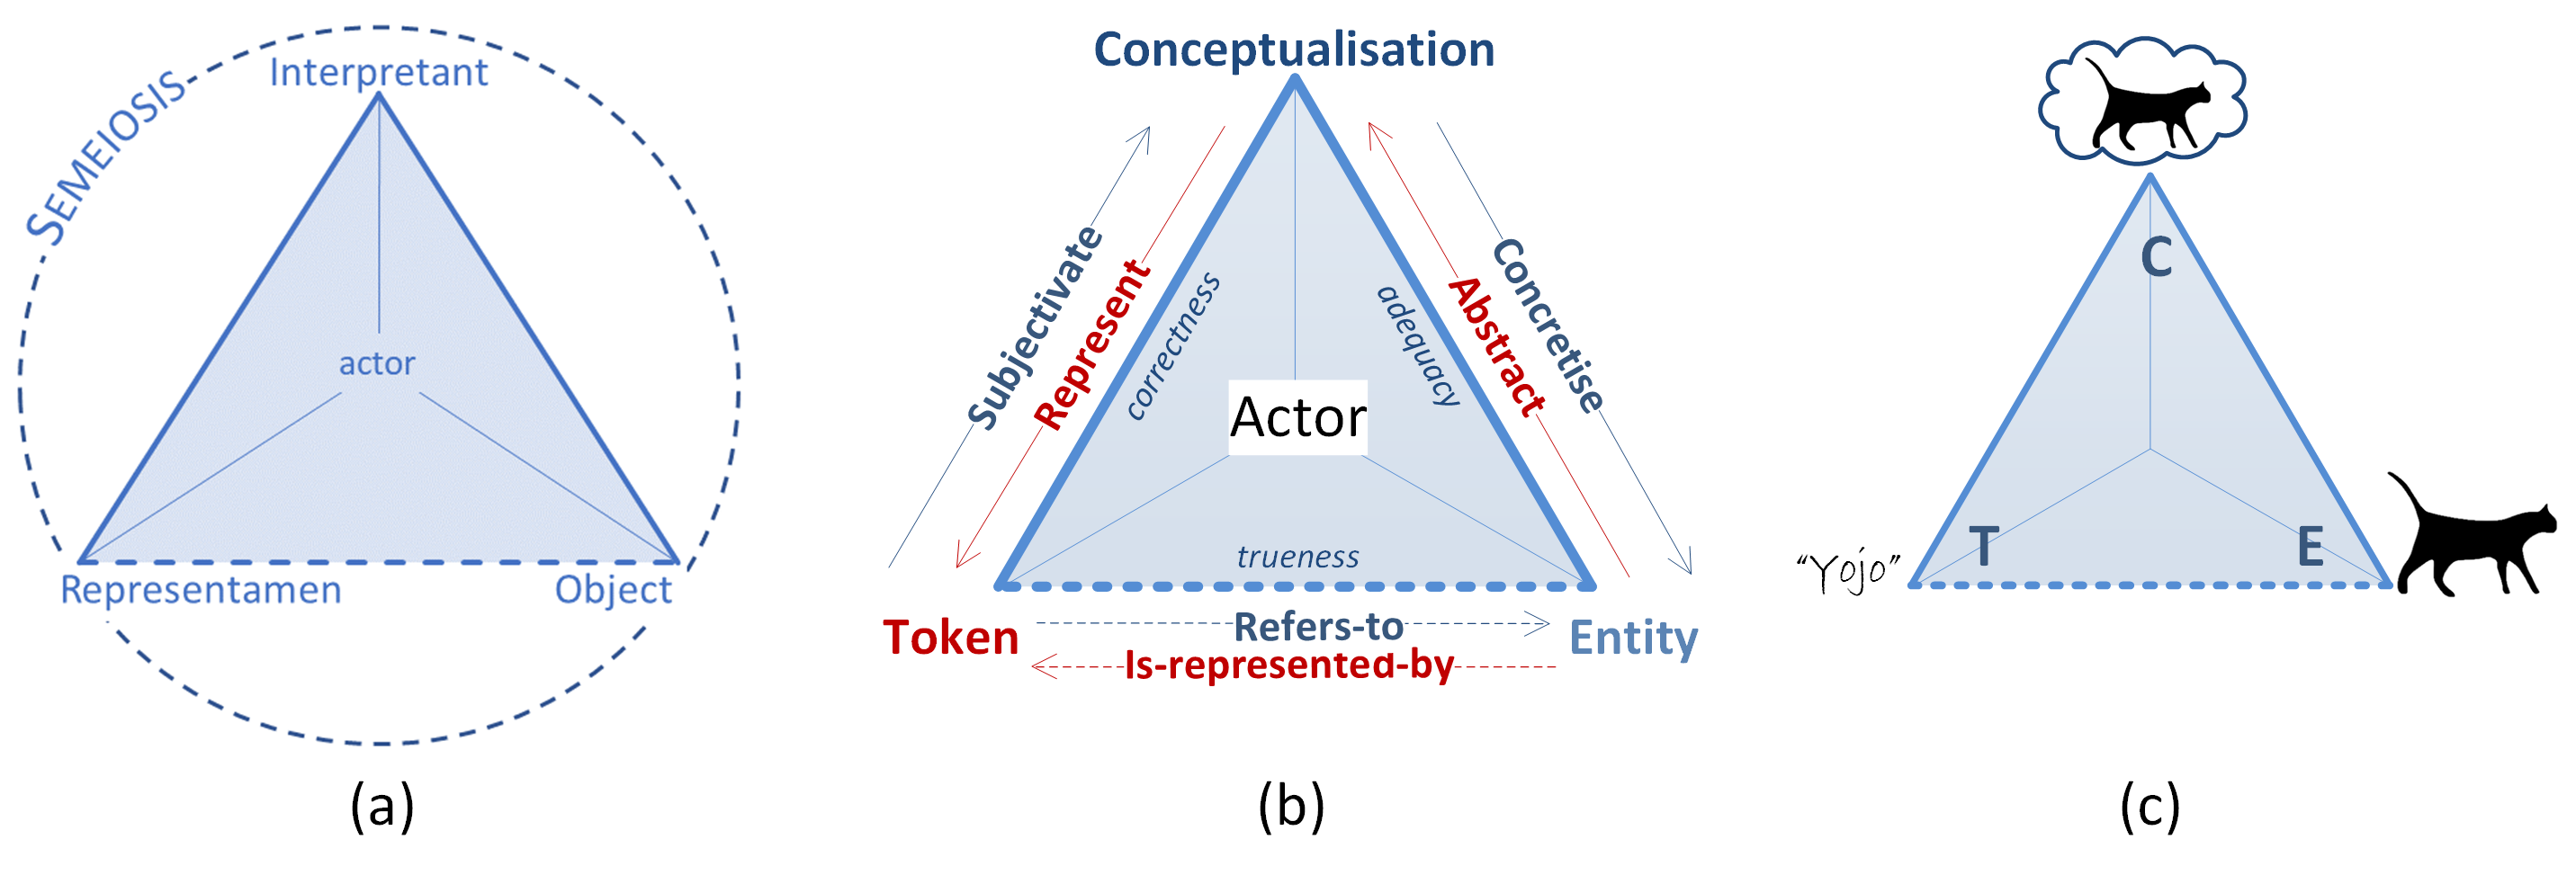
\includegraphics[width=6.25in,height=2.08333in]{src/images/SemioticTriangles.png}
\caption{The triadic model of the semiotic sign, according to Peirce
(a), and modified by us (b). Example (c) shows the concept of a cat
named ``Yojo''}\label{fig:semiotic-triangles}
}
\end{figure}

We prefer the use of \emph{entity} due to the ambiguous nature of
\emph{object} in IT. We consider an entity to stand for a thing or
event, but also a category of entities, a relation between entities and
a property of an entity. We refer to the \emph{interpretant} component
as the \emph{conceptualisation}, to underline the individual
conceptualisation that is being formed during requirements analysis and
conceptual modeling. And we prefer \emph{token} over
\emph{representamen}, and consider it both an atomic element and a
particular composition of atomic elements. We include denotations for
the edges that are connected to the conceptualisation vertex, and names
that underline the individual and mental nature of the sense making.
These names are directional, and must be read as the transformation that
takes place in that direction. Finally, we add the causal
characteristics that the edges represent, introduced by (Ogden and
Richards 1989), as \emph{adequacy}, \emph{correctness} and
\emph{trueness}. The connection between the token and the entity is a
dashed line because its existence is indirectly only through the
conceptualisation and does not exist in any direct means. With ``sign''
we mean the semiotic self-contained sign. A well-known example of a sign
is depicted in \cref{fig:semiotic-triangles}(c): when we talk about
``Yojo'', our cognition interprets it as our cat.

\begin{figure}
\hypertarget{fig:linked-triangles}{%
\centering
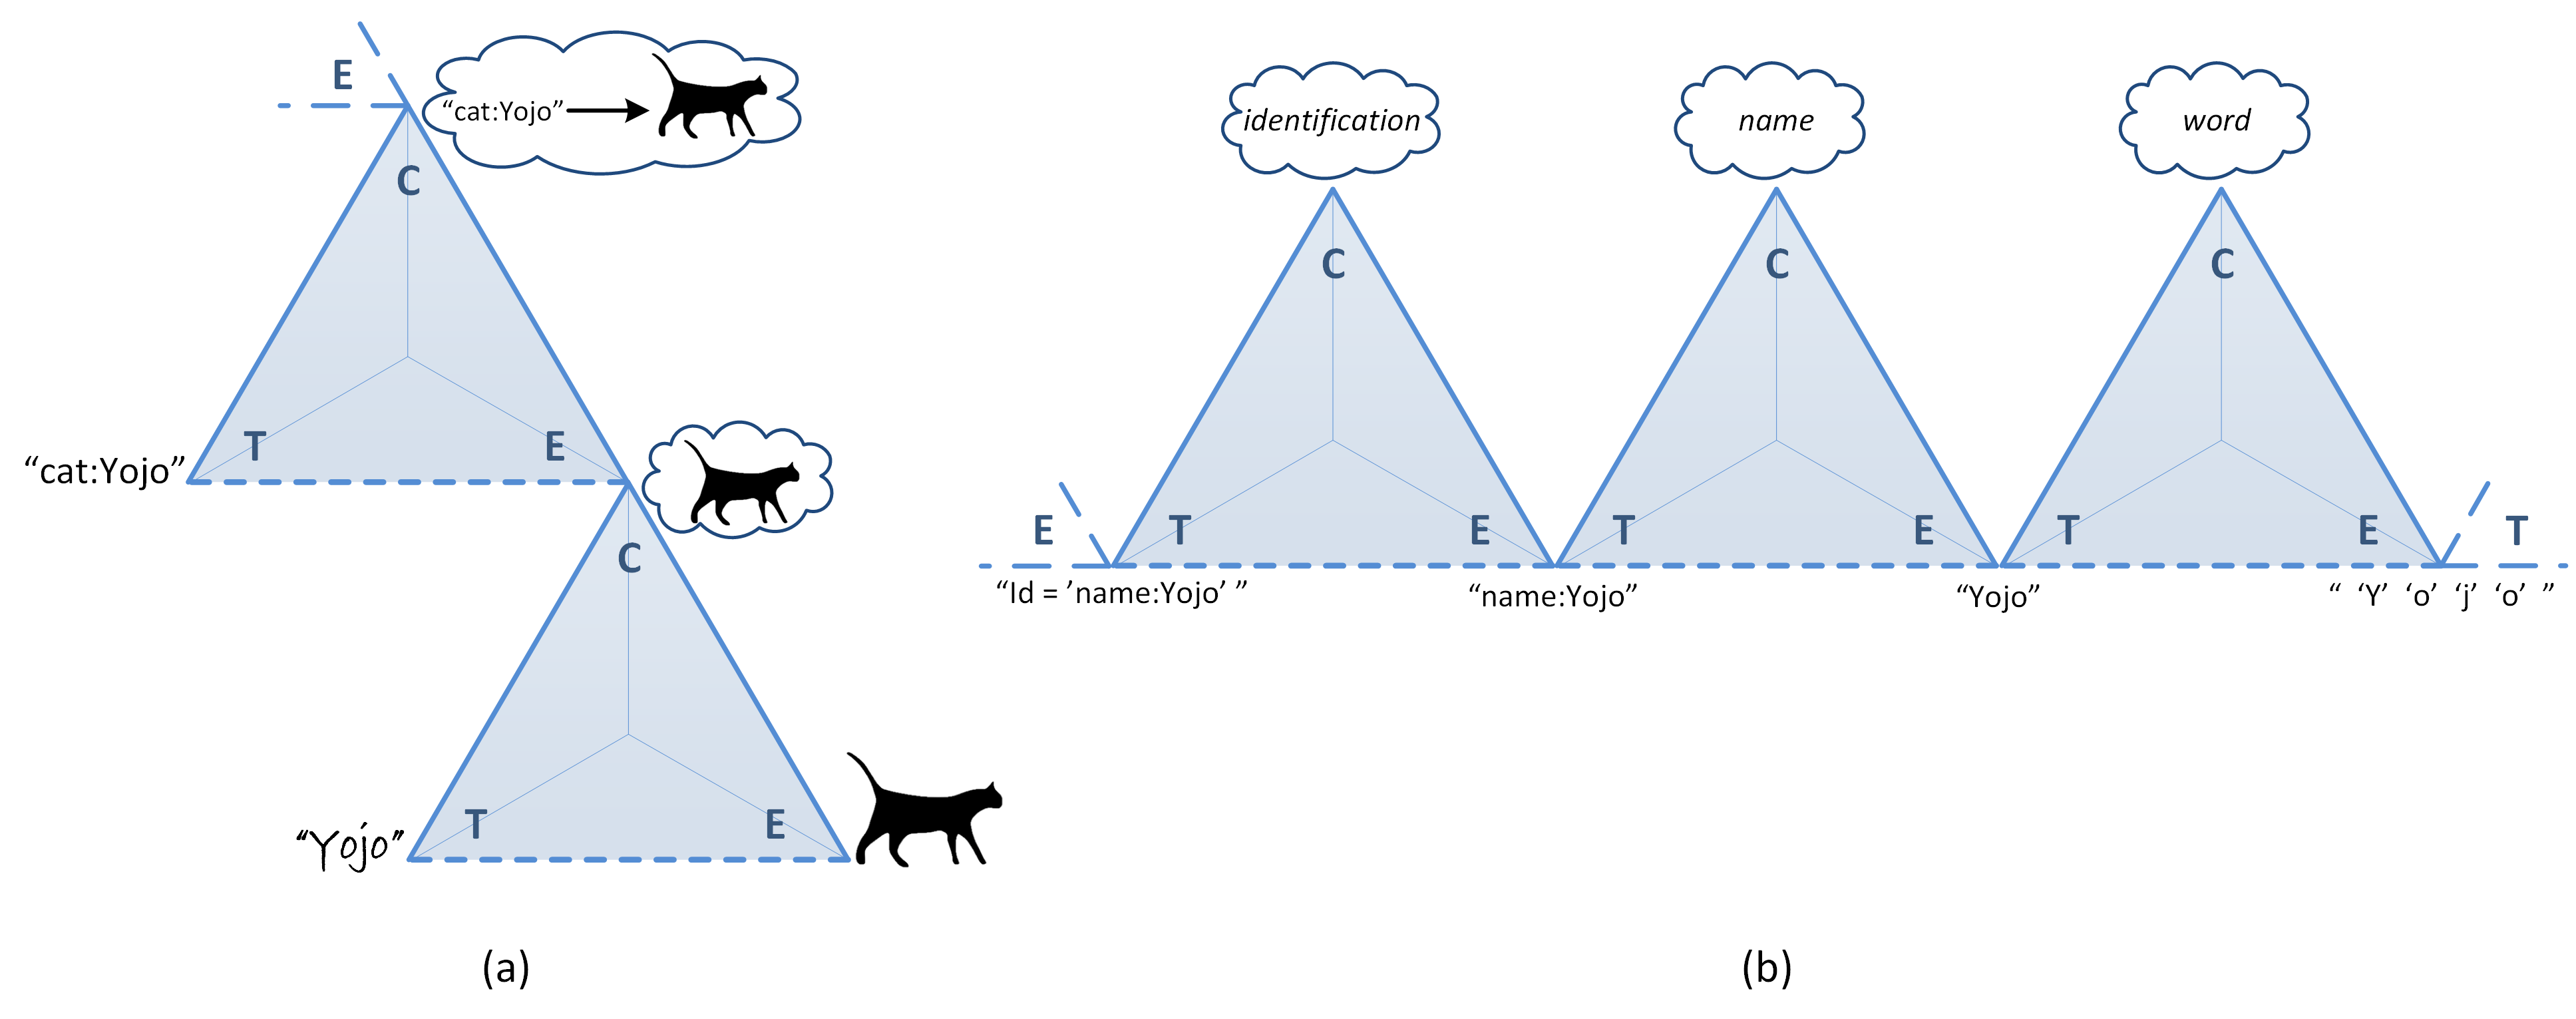
\includegraphics[width=6.25in,height=2.39583in]{src/images/LinkedTriangles.png}
\caption{Linking triadic models together.}\label{fig:linked-triangles}
}
\end{figure}

Multiple triangles can be linked together in various ways (Peirce in:
Sowa 2000). By stacking them together (\cref{fig:linked-triangles}(a)) a
conceptualisation is made of ``representing an entity'': the original
concept of a {[}\textbar{}cat{]} named
``Yojo''(\cref{fig:semiotic-triangles}(c)) is being conceptualised as
the concept of a {[}\textbar{}cat named ``Yojo''{]} and represented by
{[}\textbar{}cat:Yojo{]}. Eco (Eco 1976) uses the term \emph{unlimited
semeiosis} for the succession of stacking signs that emerge from that,
ad infinitum. We consider unlimited semeiosis as addressing a dimension
of comprehension about abstraction and generalisation, with an eventual
finish in the ultimate {[}\textbar{}Thing{]} concept.

Linking the triangles horizontally results in different representational
meta-levels, depicted in \cref{fig:linked-triangles}(b): From right to
left, the characters ``Y'' ``o'' ``j'' and ``o'' are conceptualised as a
single {[}\textbar{}word{]} and represented as ``Yojo'', which is
conceptualised as a {[}\textbar{}name{]} and represented as
``name:Yojo'', which is conceptualised as an {[}\textbar{}identifier{]}
that might be represented as ``Id='name:Yojo'''.

\hypertarget{ontological-commitment}{%
\section{Ontological commitment}\label{ontological-commitment}}

Synopsis Purpose of this section is to show the relevance of a
(modelling) language: a language is used to convey distinctions. The
distinctions that are aticulated by a language are denoted as its
ontologcal commitment. Modelling languages need to show distinctions
that are of relevance to the purpose of modelling. The predominant
purpose of modelling is to describe (a particular domain in) reality by
distinguishing the entities of interest. The ontological commitment for
a modelling language therefore should be of ontological nature,
``(\ldots{}) not in order to know \emph{what there is}, but in order to
know what a given remark or doctrine, ours or someone else's,
\emph{says} there is'' (Quine 1961). The ontological square or its
extension into the ontological sextet {[}describe it{]} can be
considered the most basic one, which have been specialized into several
flavours, all called upper-level, or top-level, or foundational,
ontologies, e.g., UFO, BFO, DOLCE and more.

Show how MDE/MDA applies an ontological commitment as defined in M3,
which facilitates an equivalent distinction as the ontological square,
but less than the ontol.sextet.

Optionally, provide for the distinctions/theories that are foundational
to the two most appropriate ontological commitments / foundational
ontologies: BFO and UFO. \textbackslash{}end\{synopsis\}

Text A (modelling) language is used to convey distinctions. The
predominant purpose of modelling is to describe (a particular domain in)
reality by distinguishing the entities of interest. The distinctions
that are thus articulated by a language are denoted as its
\emph{ontological commitment}. The ontological nature of the commitment
is characterised by: ``(\ldots{}) not in order to know \emph{what there
is}, but in order to know what a given remark or doctrine, ours or
someone else's, \emph{says} there is'' (Quine 1961).For domain analysts,
the resulting model (of the conceptualisation) represents the commitment
that the domain users have about the entities that they consider
relevant to discern: the \emph{domain commitment}. In philosophy
(Bricker 2016), similar questions are asked that relate to ``life, the
universe and everything'' as opposed to a single domain of application:
What \emph{kind} of entities exist? Are the universal aspects that seem
to be shared between individual entities, e.g.weight, taken to be
\emph{sui generis}? These are questions of ontology. From a more
pragmatic view these questions can be asked in a more constrained,
methodological nature: What kinds of entity exist \emph{according to a
given theory or discourse}? This is \emph{meta-ontology} and the answers
provide a generic framework of distinction that represents a useful
meta-model to the domain analyst, denoted the \emph{ontological
commitment. } The ontological square ({\textbf{???}}) can be considered
the most basic ontological commitment. It is obtained by considering two
formal but independent distinctions: that between \emph{types}
(\emph{Universals}) and \emph{individuals} (\emph{Particulars}); and
that between \emph{characteristics} (\emph{Properties}) and their
\emph{bearers} (\emph{Substrates}). The four resulting categories and
their causal relations are depicted in
\cref{fig:onto-square-and-sextet}(a). Its extension into the ontological
sextet (Smith 2005) is just to acknowledge that at some point the
influence of time should be incorporated as well
(\cref{fig:onto-square-and-sextet}(b)). ja, jullie gebruiken ook zoiets
(is niet OC, maar C) maar dat is te beperkt en niet gebaseerd op
realiteit (filosofie) maar op engineering sec .they can not
differentiate for example, between the cup and the coffee that is holds.
of zoClearly, similar formal distinctions can be observed in
contemporary modelling paradigms at their uppermost meta-level: OMG's
MOF M3 metametamodel distinguishes between the \emph{Association} and
the \emph{Class}, while the Resource Description Framework's language
distinguishes primarily between a \emph{subject}, an \emph{object}, and
the directed \emph{property} relation between them. All these
ontological commitments are very generic, intended to be applicable for
all circumstances. Unfortunately, being very generic, the ontological
commitments remain very sparse regarding their capability as a language
to distinguish; for all examples above, it is impossible to
differentiate, for example, between the cup and the coffee that it
holds, while intuitively, these are very different from each other. The
more extended an ontological commitment becomes, the more it can
distinguish as a language between things that we are interested in.
{[}The ontological square (a) according to ({\textbf{???}}), and its
extension (b) producing the ontological sextet according to (Smith
2005).{]}{[}def:osas{]}The ontological sextet has been specialised into
several flavours, all called \{ upper-level \textbar{} top-level
\textbar{} foundational \}\footnote{Please select the term you like
  best.} ontologies, e.g., UFO (Guizzardi et al. 2015), SUMO, YAMAYATO,
BFO, DOLCE and more, and with their similarities and differences between
them (Jansen 2008). Not all of them are intended to provide for a
complete foundation (UFO, BFO); several are only facilitating (DOLCE),
or the result of (YAMAYATO), research into particular philosophical
theories. No matter the reason for their existence, they all assume a
certain philosophical viewpoint with the purpose to accurately describe
categories that exist in reality according to their viewpoint. We
consider this the philosophical cornerstone for semantics: we can assess
the semantic validity of any proposition if and only if the underlying
ontological commitment can be referred to. Furthermore, any assessment
towards semantic interoperability of two semantic theories cannot be
made without an assessment of the similarity between their underlying
ontological commitments. Note, however, that ``We look to (\ldots{})
Ontology not in order to know \emph{what there is}, but in order to know
what a given remark or doctrine, ours or someone else's, \emph{says}
there is'' (Quine 1961). It then remains the responsibility of the
(domain) analyst or ontology engineer to select the viewpoint that is
most appropriate for its purpose, in order to select the modelling
language that describes the types of things that exist in the domain of
application the most accurate.{[}def:osas{]}:
src\images\OntoSquareAndSextet.png \{\#fig:onto-square-and-sextet
width=500px height=250px\}

\hypertarget{bridgehead-semantics}{%
\chapter{Bridgehead: Semantics}\label{bridgehead-semantics}}

Synopsis Purpose of this section:

\begin{enumerate}
\item From a semiotic perspective, explain what we mean with semantics in software agents, i.e., the reciprocity between data and data processing code (both represented as Term from the semiotic Sign).
\item Establish that for representing semantics, descriptive models (i.e., ontologies) trump prescriptive models (all 42010 models).
\item Conclude that ontologies need their place as single point of reference (trueness) in architectures, and identify their relationship with the rest of the architectures, i.e., all other prescriptive models. Note the issue on Open World Assumption (ontologies) and CWA (prescriptive models).
\end{enumerate}

\textbackslash{}end\{synopsis\}

Text

\hypertarget{what-is-software-semantics}{%
\section{What is software semantics}\label{what-is-software-semantics}}

Synopsis The purpose of this section is to explain software semantics as
the ``reciprocity between data and software code'', and show that to
some extent, set theory can replace the conceptualisation node. Conclude
that the reciprocity between data and data processing code represents
the smallest (atomic) semantic monolith.

Additionally, optionally, show:

\begin{enumerate}
\item the relationship with Grice's distinction in semantics as "what is said" and "pragmatic meaning": DONE
\item OO as initial implementation to consolidate this reciprocity, and the class as implementation of the atomic semantic monolith; 
\end{enumerate}

\textbackslash{}end\{synopsis\}

Text We take the position that weak AI is essentially a token-based
machine without the ability to close the gap between token and reality.
Also called the Grounding Problem (Harnad 1990), addressing this
fundamental issue in software engineering about semantics is at best
extremely narrow (Steels 2012), or not present at all (Cregan 2007).
This implies that the semiotic triangle is denied its conceptualisation
vertex, and the sign remains incomplete. This is confirmed by the
software engineering discipline herself implicitly, since it
consistently speaks of `models that represent reality' in a certain
purposeful context \emph{without} factoring the conceptualisation into
the equation (Aßmann et al. 2006). Consequently, the edges that connect
the conceptualisation remain vague or necessarily conflate on the
relationship between the model and reality, depicted in
\cref{fig:software-models-reality}. In terms of (Quine 1961) above, we
have beheaded the sign and cut-off our ``knowledge about our given
remark or doctrine'', we deleted that what ``we \emph{say} there is''.
We have removed the ``ontological level'' (Guarino 1994), and with that
our ``terminological competence {[}that{]} can be gained by formally
expressing the ontological commitment of a knowledge base'' (ibid.).
However, since we make do with weak AI and therefore with this beheaded
sign necessarily, we must conclude that genuine semantics can not ever
exist in current software agents.

\begin{figure}
\hypertarget{fig:software-models-reality}{%
\centering
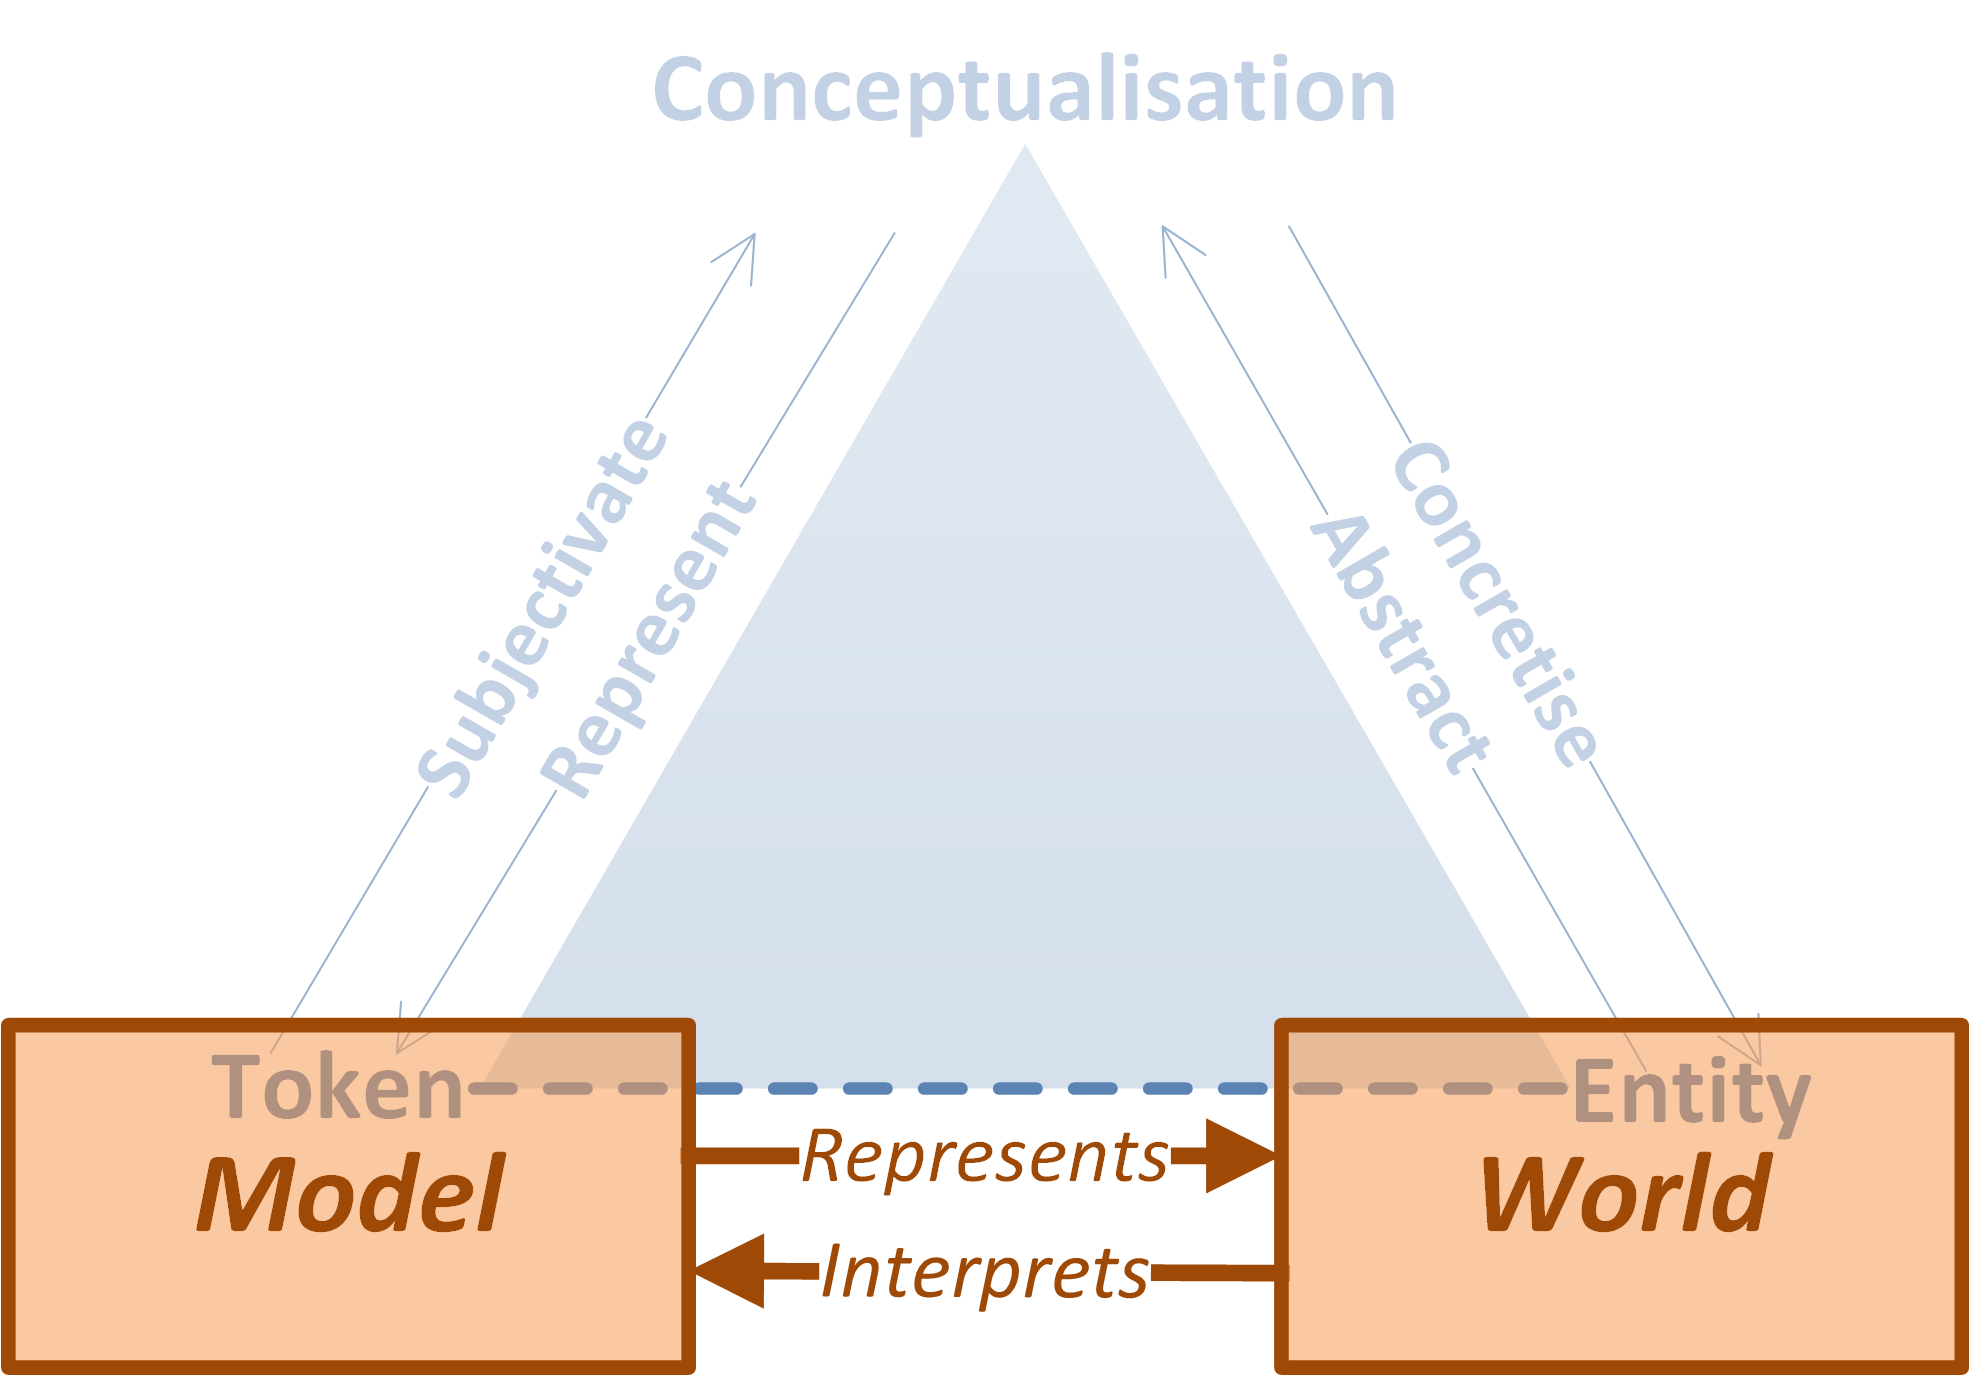
\includegraphics{src/images/SoftwareModelsReality.png}
\caption{Software engineering applies a beheaded semiotic triangle in
which its edges remain vague or conflate in the single relation between
model and reality.}\label{fig:software-models-reality}
}
\end{figure}

During the use of a software agent the semeiosis is taken care of by the
human-in-the-loop, viz. the end user at the human-machine interface
(HMI) whom interprets the tokens that are displayed (subjectivation).
During development of a software agent the semeiosis is taken care of by
another human-in-the-loop, viz. the software engineer whom implicitly
performs the conceptualisation and explicitly represents this
conceptualisation into tokens, i.e., \emph{models}. Consequently, all
models are representations of the engineers' conceptualisations. From
the many models that software engineering typically generates we focus
on a pair of models that constitute the engineers' semantics: the
information or data models{[} brandtp, 8/30/2018 Make use of 42010
terminology{]} that refer to the \emph{information entities} in reality,
paired with the process or business models{[} brandtp, 8/30/2018
\ldots{} ditto \ldots{}{]} that represent the \emph{event entities} that
operate on the information entities. Data processing is in its bare form
nothing more than tokens that follow a specific language grammar. This
bare form is a representation of its quintessence, viz. a run-time
notion on the proper way to operate on the data. Together, these models
comprise the smallest atomic union that can represent meaning, indicated
by (Grice 1989) as a twofold: the \emph{semantic} meaning, or ``what is
said'', and the \emph{pragmatic} meaning, what we like to understand as
``how it relates to our intentions''.

\begin{mmdef}[Atomic semantic monolith]\label{def:atomic-semantic-monolith}
An Atomic Semantic Monolith (ASM) denotes the smallest, highest grained pair of models (a data model and a data processing model) that remains faithful to the entity in reality that it refers to.
\end{mmdef}

At the modelling level, semantics still exist by virtue of the designer.
However, when the software agent is subsequently compiled, its binary
code originate from the process model of the model pair (operations,
algorithms), and the memory allocation for the data originates from the
information model of the model pair (size, format, encoding). At this
binary level the software engineer has left the building, and with her
the conceptualisation vertex and the subsequent capability for semeiosis
and, thus, semantics. In other words, at binary level we have lost the
capability to verify the semantic coherence between the code and the
data while the reciprocity between data and software code determines the
semantic validity of the data processing. For instance, consider a data
element \(t\) to represent temperature, and a data algorithm to
establish fever, e.g., \texttt{t\ \textgreater{}\ 37.0} \(\to\)
\texttt{fever}. The one and only means to keep the software from failing
is that both the data and the algorithm (i) are expressed in the same
unit of dimension (\(\si{\degree}C\) in this example), apply the same
(ii) resolution and (iii) accuracy, to name a few obvious constraints.
We, therefore, take the stance that semantics can only exist in software
by virtue of the semeiosis by the human-in-the-loop, while in the
software agent itself semantics are necessarily reduced to the
reciprocity between data and software code. Still, the software agent
acts as transport medium for the semantics as intended by the software
engineer to the semantics as experienced by the end user at the HMI. We
therefore consider the coherence between data models and data processing
models essential for enforcing the software agent to maintain a semantic
valid reciprocity between binary code and the data it operates on.

This leads to the definition of a (normative (Greefhorst and Proper
2011)) design principle to its effect:

\begin{mmdp}[Semantic coherence principle]\label{dp:semantic-coherence-principle}

Establish explicit coherence between the models that are contained in a semantic monolith.

\textbf{Type of information:} business

\textbf{Quality attributes:} (semantic) accuracy, reusability, manageability, understandability 

\textbf{Rationale:}
\begin{enumerate}
\item Semantics in software agents are necessarily reduced to, and emerge from, the reciprocity between the data and the binary code that operates on them;  
\item Without explicitly addressing -- at modelling level -- \textbf{all} facets that influence the coherence between the data on the one hand, and the operations that apply on them on the other, the software agent cannot guarantee to maintain the reciprocity between them at the binary level;
\item Without maintaining the reciprocity between binary code and the data it operates on, the semeiosis performed by the end user on the result of the data processing and their subsequent semantics cannot be guaranteed to be similar as intended by the software engineer.
\end{enumerate}
\textbf{Implications:}
\begin{enumerate}
\item The coherence principle is a necessary condition for supporting semantic interoperability;
\item The scope of semantic validity \& accuracy is addressed explicitly and can be referred to;
\item Reuse of data often implies reuse of the data processing code, and vice versa. Having established explicit coherence improves the quality of data and code reuse, and facilitates the verification that the scope of the semantic validity \& accuracy applies in the new context as well;
\item manageability ...?
\item understandability ...?
\end{enumerate}  
\end{mmdp}

Coherence between models can be established with use of a single unique
reference against which the truth of the expressions of both models can
be verified. In semiotics, this single unique reference is considered
reality, as indicated in \cref{fig:semiotic-triangles}(b) by the
\emph{trueness} characteristic. Except as toy example in (Steels 2012),
this is clearly not possible. The \emph{correctness} characteristic is
the only alternative left, taking the conceptualisation node as its
principle point of reference, as depicted in
\cref{fig:single-semantic-reference}(b). This is exactly what the
mathematical branch of \emph{formal semantics} achieves (Gamut 1991;
Genesereth and Nilsson 1987) with its three main characteristics,
depicted in \cref{fig:single-semantic-reference}(a), viz. connecting (i)
an abstract syntax of a language to (ii) a domain of interpretation
(usually a set theoretic framework) by defining (iii) an interpretation
function from the abstract syntax onto the set theoretic framework. In
terms of the semiotic triangle, \cref{fig:semiotic-triangles}(b), this
implies the following:

\begin{enumerate}
\def\labelenumi{(\roman{enumi})}
\tightlist
\item
  the \emph{representation} node represents models that can be
  formulated by use of an abstract syntax (and grammar) as its modelling
  language. In this reading, a model is a particular constellation of
  tokens that represent a particular state of affairs;
\item
  a particular \emph{conceptualisation} can be mathematically formulated
  as a specific constellation of (unnamed) individuals, sets of
  individuals, and sets of sets;
\item
  the \emph{subjectivation} edge can be formulated as the interpretation
  function that assigns a mapping from modelling language tokens onto
  the set elements, enabling the evaluation of a specific model against
  the intended conceptualisation from (i).
\end{enumerate}

In this way, the cognitive quality of the conceptualisation can be
substituted with set theory. Formulating the conceptualisation as a set
theoretic model essentially remains a representation, albeit a
mathematical one. One can argue that such substitution does not resolve
the grounding problem, and appropriately so. Still, mathematics provide
for a very exact way to express oneself, reducing the ambiguity that
comes implicitly with any other language, and such mathematical
constructs come as close to the conceptualisation as we possibly can get
with a token-based machine. Furthermore, logical constructs used at the
syntactical level can be interpreted into set theoretic operations,
facilitating the evaluation of (complicated) expressions. Formal
semantics thus provides a domain of discourse about a particular
conceptualisation as principle point of reference for both the data
model and the data processing model. The particular conceptualisation is
then replaced with a particular Domain of Interest (DoI), and both
subjectivation relations are replaced with their interpretation function
on the abstract syntax of the models.

\begin{figure}
\hypertarget{fig:single-semantic-reference}{%
\centering
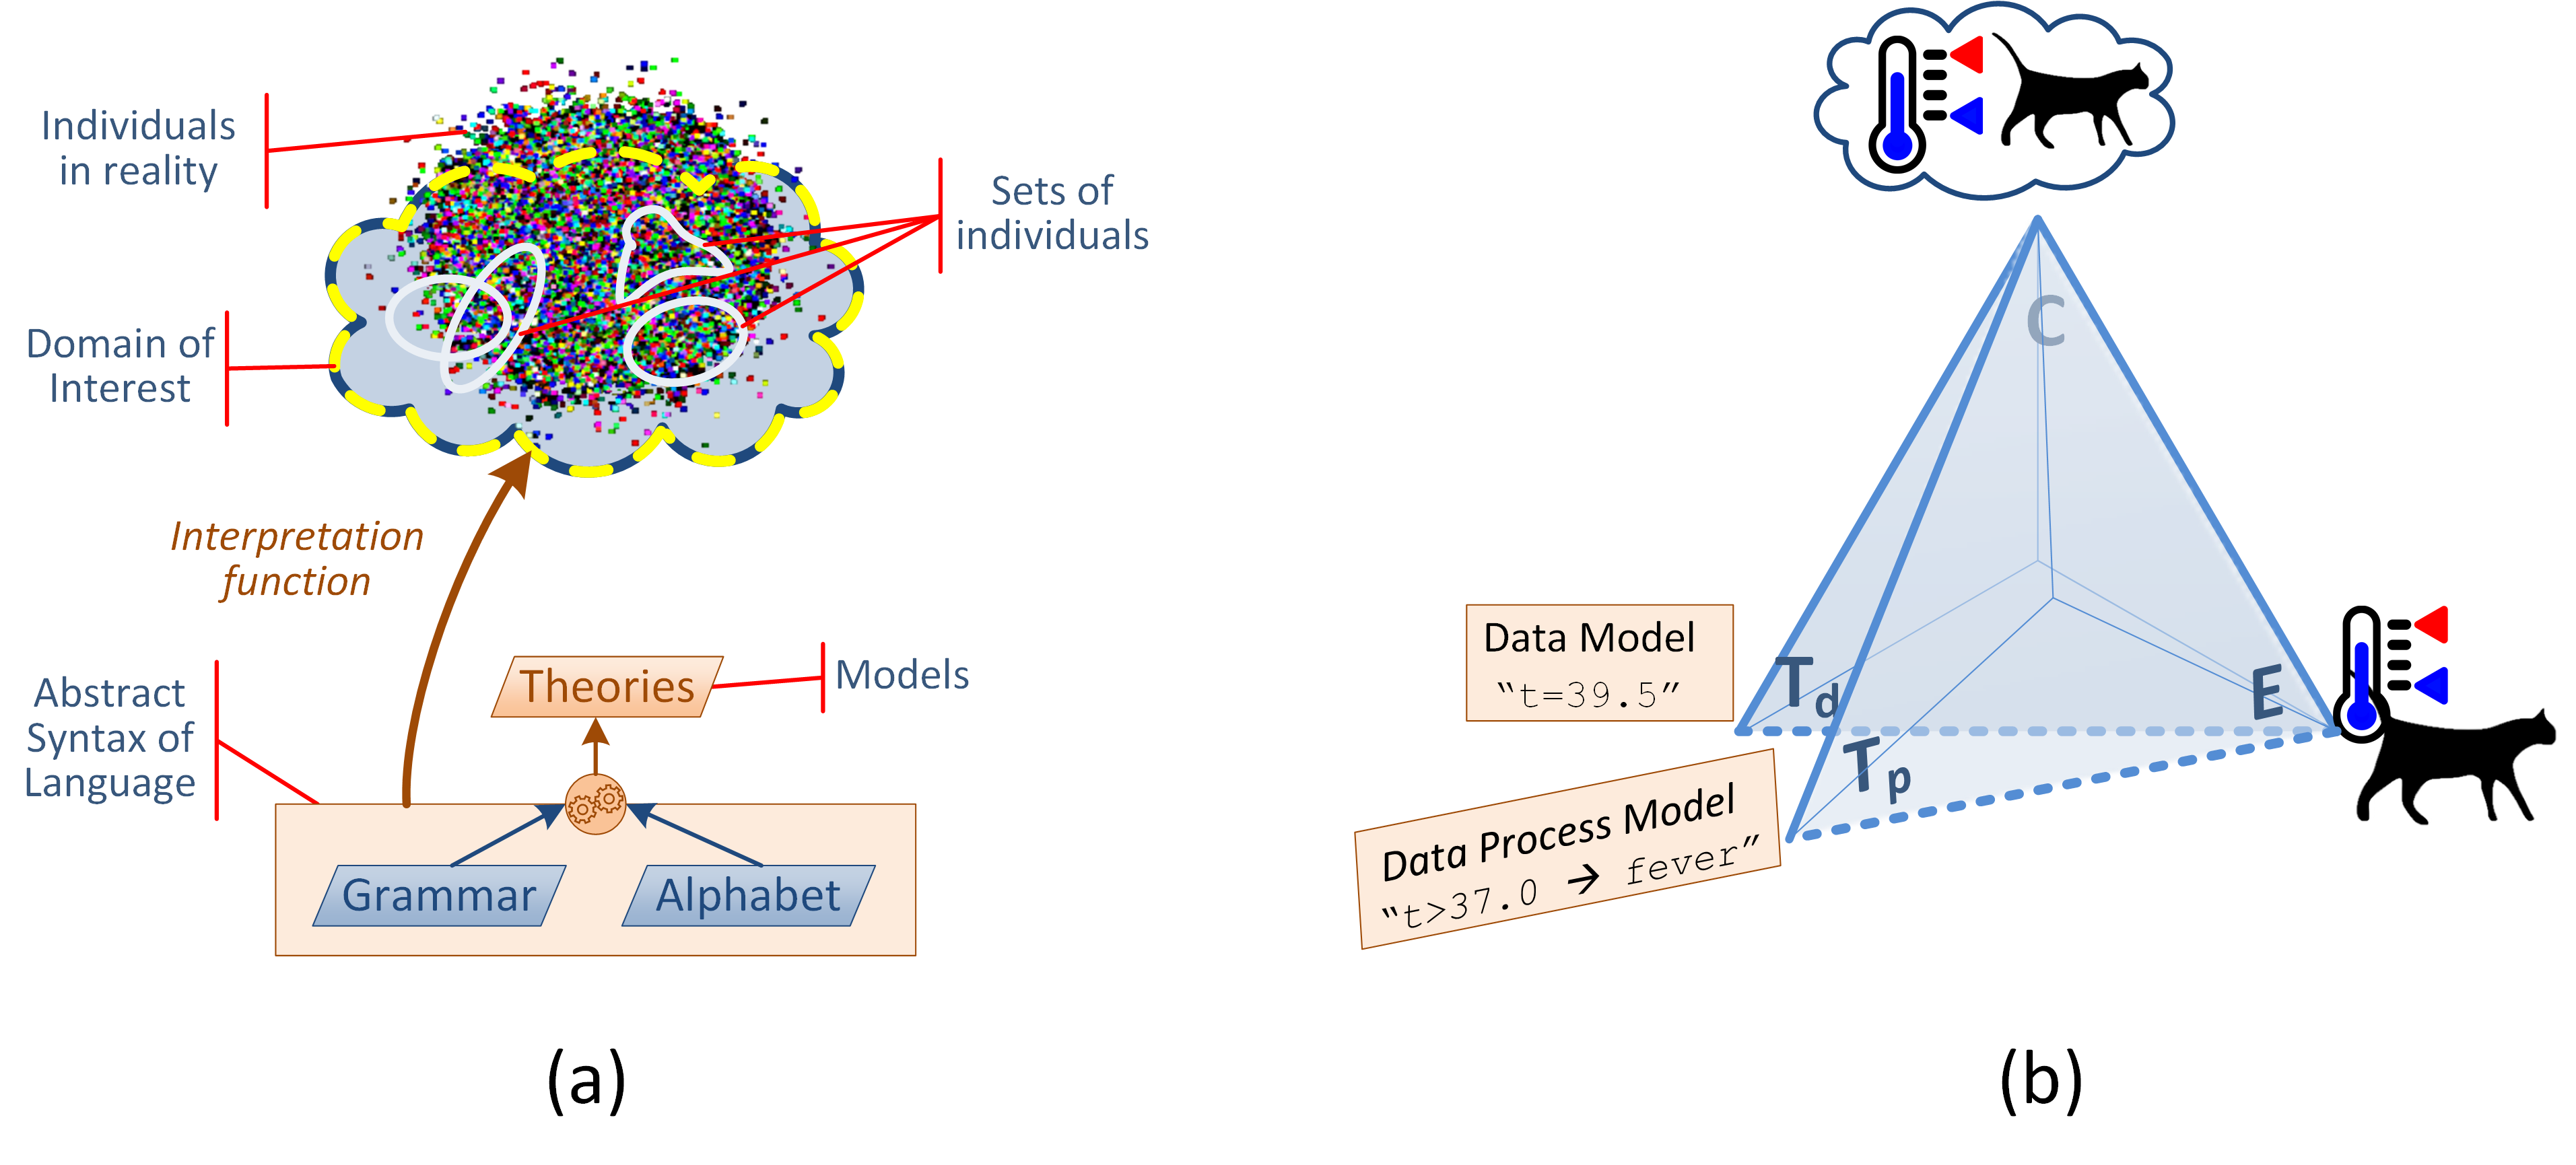
\includegraphics{src/images/SingleSemanticReference.png}
\caption{Maintaining the reciprocity between data and data processing
models through a single semantic reference, viz. the conceptualisation
(b), represented as DoI, viz. a selection of individuals with domain
specific characteristics defined as sets
(a).}\label{fig:single-semantic-reference}
}
\end{figure}

In conclusion, we explain software semantics as the reciprocity between
data and software code, realised by maintaining the coherence between
pairs of data and data processing models, by applying formal semantics
to formulate a particular conceptualisation as a DoI that can act as
semantic reference, and interpretation functions which perform the
subjectivation from the data and operation models to that reference.

\textless{}2nd Principle: Make the ASM as small as possible, but not
smaller than required to express a semantic element. Too vague, yet. Not
necessary to convey the primary message, imo.\textgreater{}

\textless{}Elaborate on OO to consolidate the reciprocity; take the
class as example of a semantic monolith, the minimal, atomic
one.\textgreater{}

\hypertarget{explicit-semantics}{%
\section{Explicit semantics}\label{explicit-semantics}}

Synopsis The purpose of this section is to establish that for
representing semantics, descriptive models (i.e., ontologies) trump
prescriptive models (all 42010 models)

Firstly, describe that formal semantics can to some extend take the role
as conceptualisation, and hence using set theory as conceptualisation is
the best option we have to address semantics. Consequently, show that
semantic ambiguity then ``only'' follows from 4 construction issues
(already presented in text below).

Secondly, make the distinction between descriptive and prescriptive
models (Henderson-Sellers 2012), and in (Aßmann et al. 2006):
``Specification models focus on the specification, control, and
generation of systems; ontologies focus on description and
conceptualization (conceptual modelling) of things. Both kinds of models
have in common the qualities of abstraction and causal connection.''

Second argument shows that (i) the trueness of a model is laid in
reality, which is impossible to achieve, and that (ii) the next best we
can achieve is establishing the correctness of a model against its
conceptualisation node. Finally, observe that (iii) 4 issues will
influence the correctness of the model. Then conclude that the best tool
to control these issues are the logics from descriptive models (viz.
ontologies) at the one hand, and its use as ontological commitment for
the prescriptive models (viz. the 42010 models)

Conclusions:

\begin{enumerate}
\item ontologies are more appropriate artefacts for conceptual models than system models
\item as in [@Aßmann2006]: "Specification models focus on the specification, control, and generation of systems; ontologies focus on description and conceptualization (conceptual modelling) of things. Both kinds of models have in common the qualities of abstraction and causal connection."
\end{enumerate}

\textbackslash{}end\{synopsis\}

Text Once we have established a conceptualisation, it needs a
representation because, despite being a mathematical representation, the
sets and individuals in the DoI remain nameless. It is necessary to
represent them in a (pair of) model(s) that is tangible, computational
and a distinct artifact in order for the software agent to use it and,
eventually, make comparisons with the semantic artifact of the peer
software agent. We denote the model that represents a conceptualisation
a \emph{conceptual model}. The conceptual model that describes semantics
best is a model that is as faithful to reality as possible. This begs
the questions about the nature of a conceptual model and the nature of
faithfulness. To start with the latter and as indicated in
\cref{fig:semiotic-triangles}(b), we equate faithfulness with trueness
between the representation and the entity in reality. Since this aspect
is a characteristic of an indirect relationship, it can only emerge as a
result of the adequacy and correctness characteristics. The former one
concerns the conceptualisation aspect; in this section we address the
correctness and show how differences can emerge between the
conceptualisation and the model when constructing the latter. In
literature, four construct issues are considered between a
conceptualisations and its representation in a model, depicted in
\cref{fig:construct-issues}. An exhaustive treatment can be found in
(Guizzardi 2005), see also (Carvalho e Silva et al. 2012; or Azevedo et
al. 2015).

\begin{figure}
\hypertarget{fig:construct-issues}{%
\centering
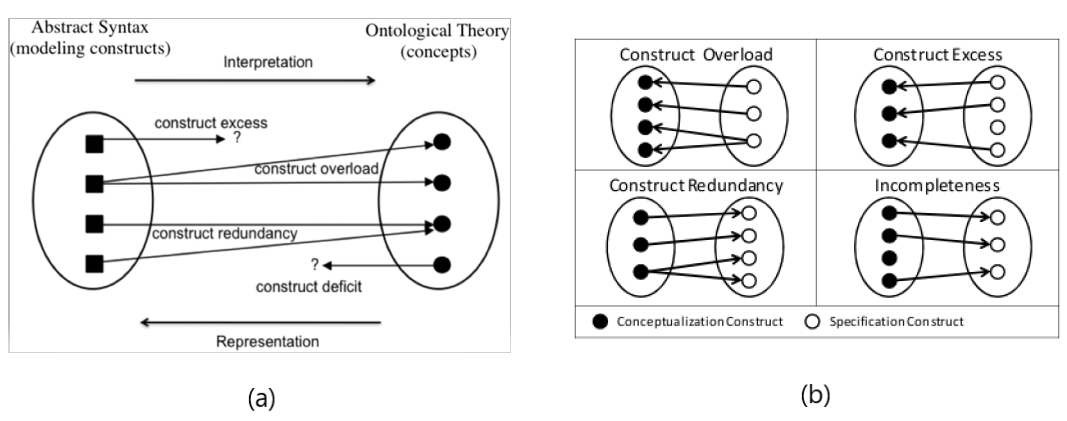
\includegraphics[width=5.55208in,height=2.1875in]{src/images/ConstructIssues.png}
\caption{Four different types of construction issues that come with
formal semantics. Which one is more clear: (a)(Carvalho e Silva et al.
2012) or (b) (Azevedo et al. 2015)?}\label{fig:construct-issues}
}
\end{figure}

The more precise the representation of the conceptualisation, the higher
its \emph{comprehensibility appropriateness{[} *brandtp, 9/19/2018
describe/explain the term{]}}.* Semantic accuracy improves when
minimising the four construct issues:

\begin{itemize}
\tightlist
\item
  \emph{Construct overload}, or \emph{non-lucidity}, emerges when the
  interpretation function maps an element from the abstract syntax onto
  more than one element (individual, subset) from the conceptualisation:
  One token can mean more than one thing, e.g., {[}\textbar{}bank{]};
\item
  \emph{Construct excess}, or \emph{unsoundness}, represents an abstract
  syntax element that does not map onto an element from the
  conceptualisation: One token does not have a meaning at all;
\item
  \emph{Construct redundancy}, or \emph{non-laconicity}, occurs when
  more than one abstract syntax element can be used to represent an
  element from the conceptualisation: More tokens mean the same, e.g.,
  \ldots{}{[} brandtp, 9/19/2018 find proper example{]};
\item
  \emph{Construct deficit}, or \emph{incompleteness}, specifies the
  situation where a conceptual element does not map onto a token: It is
  impossible to express a concept because the language has no token for
  it, e.g., {[}\textbar{}\ldots{}.{]} (example intentionally left
  blank).
\end{itemize}

The best representation of a conceptualisation, then, is a model that is
lucid, sound, laconic and complete, i.e., the
interpretation/representation mapping is isomorphic. This is difficult
to achieve, and due to the complete, accurate and complementary
categories of how its carves-out the DoI, using the ontological
commitment of the modelling language proves a useful tool in that
respect.

In contemporary architectural paradigms, models are being used as first
class citizens to the architectures, MDA, IEEE-1471 and ISP RM/ODP
alike. It is therefore imperative to decide upon the major
characteristics of a model. The distinction between descriptive and
prescriptive models is broadly accepted, where a prescriptive model is
used to \emph{specify} its subject, and a descriptive model is used to
\emph{describe} its subject. As explained by (Gonzalez-Perez and
Henderson-Sellers 2007), this distinction only addresses how the model
is being used and does not express a complementary, disjunct property.
In stead, a genuine dichotomy emerges when considering the \emph{role}
that the model plays (ibid.). Then, a specification model generally
takes a forward-looking role, specifying how the subject is supposed to
be. A descriptive model, on the other hand, generally takes a
backward-looking role and addresses the subject as it currently is, or
once has been. In (Aßmann et al. 2006), the relationship that a
forward-looking model has with its subject is characterised as an
\emph{instance-of} relation, and that of a backward-looking model as an
\emph{is-represented-by} relation. Although we acknowledge the
differences that exist, we consider both terms confusing when semiotics
are involved since we cannot substantiate their suggested equivalence
with the instantiation relation from the ontological square/sextet or
the representation relation from the semiotic triangle. Instead, we
observe that the characteristics of the \emph{refers-to} relation will
specialise into a \emph{declarative} relation for a forward-looking
model: The entity is deemed to follow the rules that are specified by
the model. Similarly, for a backward-looking model that provides for a
representation of ``what a given remark or doctrine, ours or someone
else's, \emph{says} there is'', the refers-to relation specialises into
a \emph{descriptive} relation. We thus observe that the refers-to
relation is a causal relation, the direction of which is dependent on
the model's characteristic: declarative towards the entity for a
forward-looking model, while descriptive towards the token for a
backward-looking model. As a consequence, we conclude that for
forward-looking models their truth lies in their meta-models, as
depicted in \cref{fig:linked-triangles}(b). Mutatis mutandis, the truth
for backward-looking models lies in the entities they describe.

\begin{enumerate}
\def\labelenumi{\arabic{enumi}.}
\tightlist
\item
  Explain: difference between ontologies and models

  \begin{enumerate}
  \def\labelenumii{\roman{enumii}.}
  \tightlist
  \item
    Models lack an elaborate ontological commitment, domain ontologies
    naturally evolve on foundational ontologies (that express an
    ontological commitment)
  \item
    For prescriptive models, truth lies in meta-models (good for
    deterministic behaviour); ontologies are descriptive models for
    which the truth lies in reality (good for semantics)
  \item
    ontologies have open world assumption (semantic
    under-specification), models have closed world assumption (data
    remain consistent, good for performance)
  \item
    Models specify systems, ontologies conceptualise reality (entities)
  \end{enumerate}

  \begin{itemize}
  \tightlist
  \item
    Try to also connect the onto/model distinction with above principles
  \item
    Induced problem: from OWA (domain ontologies) to CWA
    (information/data models), viz. how to get closure?
  \item
    Principle: use domain and business ontologies for ``computational
    independent''-ish models (Aßmann et al. 2006)
  \item
    Bridge descriptive --\textgreater{} prescriptive models by grounding
    all prescriptive model elements with concepts from descriptive model
    (see e.g. \cref{fig:OntosInMDE}).
  \end{itemize}
\end{enumerate}

In the remainder of this text we will refer to the formulation of the
reference conceptualisation as a \emph{conceptual model}.

\begin{figure}
\hypertarget{fig:OntosInMDE}{%
\centering
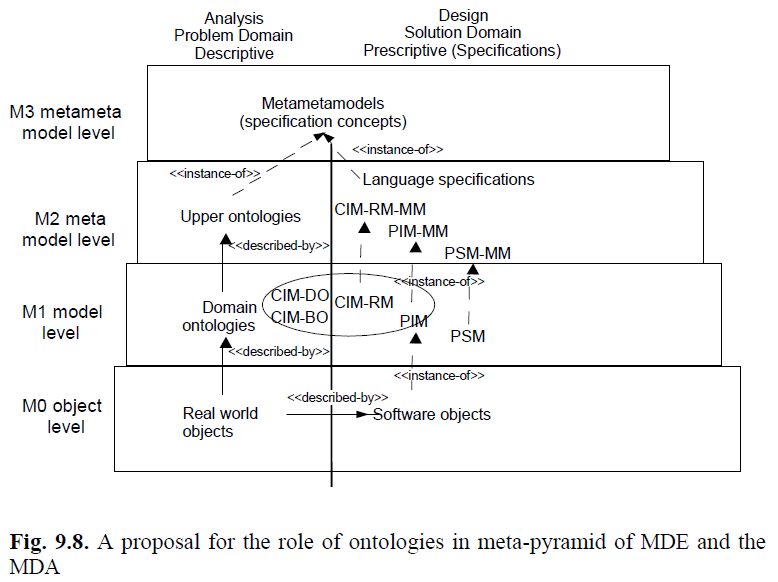
\includegraphics[width=5.91667in,height=3.60417in]{src/images/OntosInMDE.png}
\caption{The use of ontologies in MDA, from (Aßmann et al.
2006)}\label{fig:OntosInMDE}
}
\end{figure}

\hypertarget{spanning-alignments}{%
\chapter{Spanning: Alignments}\label{spanning-alignments}}

\hypertarget{what-is-semantic-interoperabiity}{%
\section{What is semantic
interoperabiity}\label{what-is-semantic-interoperabiity}}

Synopsis

\begin{enumerate}
  \item Explain sIOP:
  \begin{enumerate}
    \item that consequence of data exchange = breaking the atomic semantic monolith = breaking the reciprocity by partitioning the data from its original code, and explain that standards are large semantic monoliths that roofs that point but are as manouverable as an oil tanker, and 
    \item that sIOP demands that despite this partitioning the reciprocity between the code of the receiving agent and the external data shall be re-installed.
    \item Optionally, give a definition on phantom semantics
  \end{enumerate}
  \item We therefore need to extend the semantic coherence Principe into a sIOP coherence principle with a sIOP rational that the result of the semeiosis on receiving agent A’ does not conflict withthe outcome of the semeiosis on agent A: Without maintaining the reciprocity between binary code and the data it operates on, the semeiosis performed by software engineer A’ on the result of the data processing and their subsequent semantics cannot be guaranteed to be similar as intended by the software engineer.
  \item Explain the difference with semantic standards which are basically large semantic monoliths
  \item Introduce Principle: ontological commitment as minimal standard for sIOP, “(...) not in order to know *what there is*, but in order to know what a given remark or doctrine, ours or someone else’s, *says* there is” [@Quine:1953er]
\end{enumerate}

\textbackslash{}end\{synopsis\}

Text Rephrase: despite the notoriously difficult philosophical questions
involved, semantic interoperability can be seen as an engineering
problem, namely that of effectively constraining interpretations towards
the ones that are considered allowable (Kuhn 2009).

\begin{figure}
\hypertarget{fig:2semiotic-triangles}{%
\centering
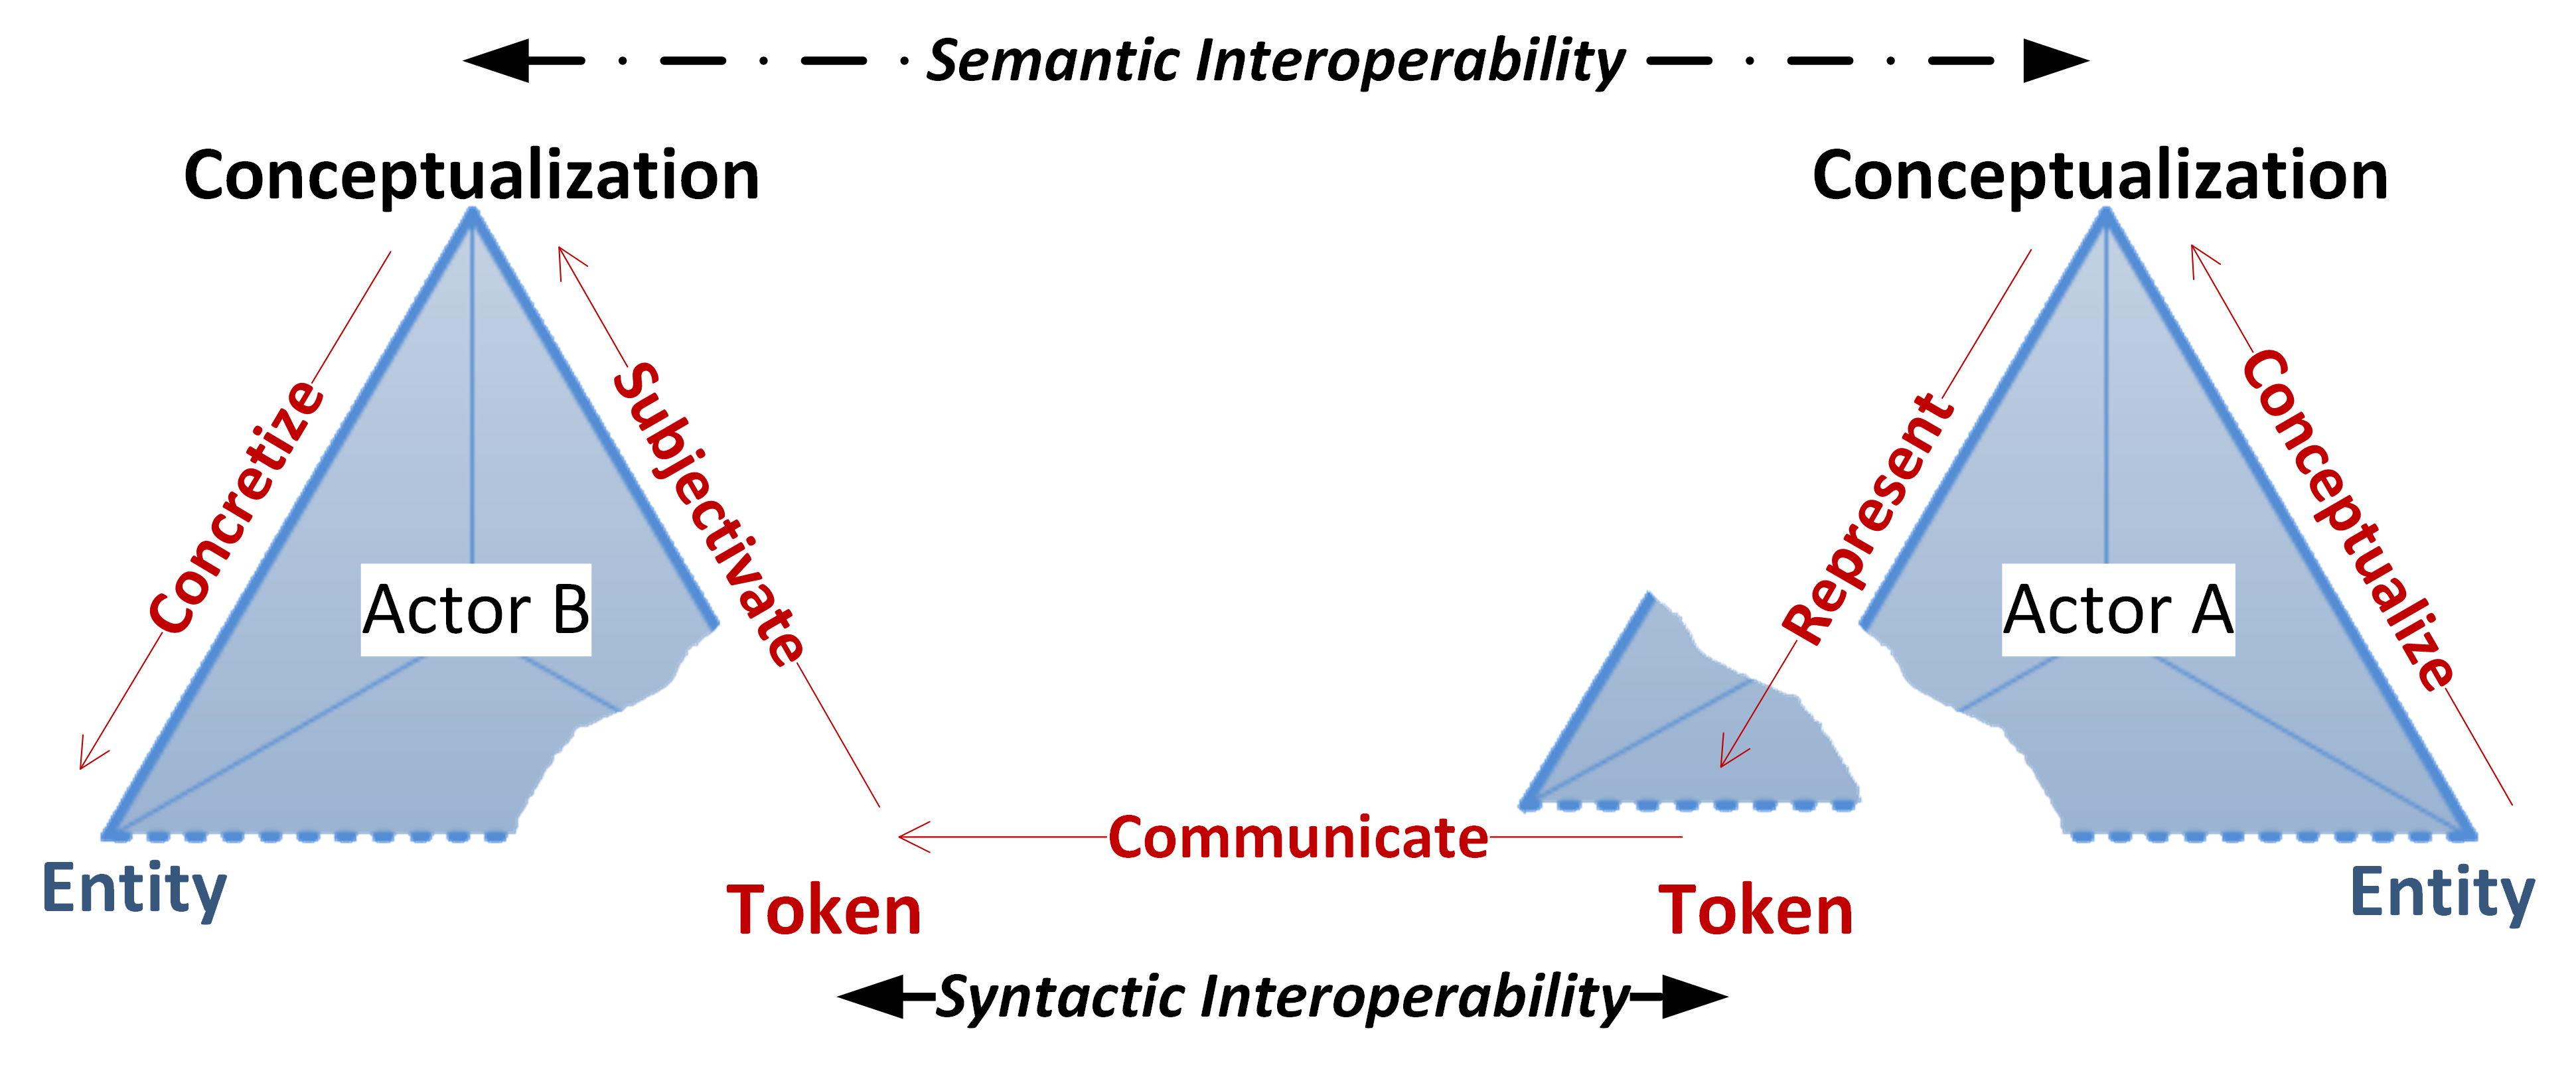
\includegraphics[width=5.3125in,height=2.25in]{src/images/2SemioticTriangles.png}
\caption{The various forms of
interoperability}\label{fig:2semiotic-triangles}
}
\end{figure}

\hypertarget{expicit-siop-by-alignments}{%
\section{Expicit sIOP by alignments}\label{expicit-siop-by-alignments}}

Synopsis Thus:

\begin{enumerate}
\item Follow the coherence principle and conclude that the models from which *external* data and *receiving* data processing code are derived, need to be brought into coherence with each other.
\item The coherence principle already enforced a single unique reference for each agent. Re-installing coherence demands a semantic alignment between those single unique references. 
\item The purpose of that alignment is to establish how the truth of expressions that are formulated in terms of agent A, can be estabished by using formulations in terms of agent A' against the single unique reference from A'. 
\item The language that is used for expressing the alignment should be fit for its purpose. Refer to EDOAL [@Scharffe2011] as the currently most complete one.
\end{enumerate}

\textbackslash{}end\{synopsis\}

Text

\begin{figure}
\hypertarget{fig:3Concerns}{%
\centering
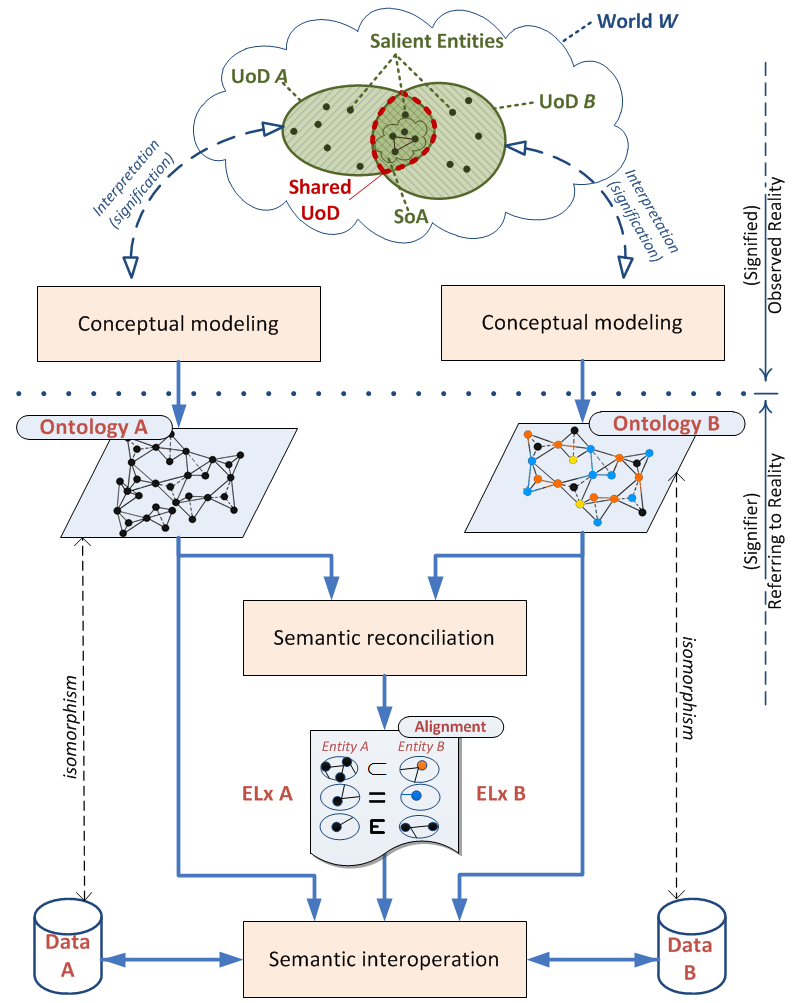
\includegraphics[width=5.15625in,height=7.21875in]{src/images/3SemanticConcerns.png}
\caption{The three semantic concerns are related: conceptual modelling,
semantic reconciliation, and semantic mediation}\label{fig:3Concerns}
}
\end{figure}

\hypertarget{roadway-mediation}{%
\chapter{Roadway: Mediation}\label{roadway-mediation}}

Synopsis Purpose of this section: Establish requirements for a
\emph{generic} mediator.

With mediation we denote the process of transcribing a data term that
originates from Agent A into a data term that matches a term familiair
to Agent A', based on both agents' ontologies and the alignment between
them. The main issue here is that although many different types of
relation can be defined between the concepts of ontology A and A', e.g.,
superset of, a transcription of a token from A into a token from A' is a
complete replacement and, hence, implements an equivalence relation. In
(Brandt et al. 2018), we show a semantic valid transcription process.
The requirements of a mediator are:

\begin{enumerate}
\item Being a generic service
\item Fully defined by two ontologies and their alignments
\item Allows for semantic valid transcriptions only, where 'validity' refers to absence of inducing phantom semantics.
\item Appropriate behaviour for non-translatable content, which should apply only as result of an incomplete alignment, a logical incorrect alignment, or attempts to communicate content that is considered irrelevant for the receiving agent.
\end{enumerate}

\textbackslash{}end\{synopsis\}

\hypertarget{siop-principles}{%
\chapter{sIOP Principles}\label{siop-principles}}

Synopsis Purpose of this section:

\begin{itemize}
\item Show the semantic architecture as an additional layer that is orthogonal to current layers, expressing a separation of concerns between syntax and semantics (see [@Brandt:2013jh])
\item Define loosely coupled semantics as a result of applying the 2 principles 'semantic separation of concerns' and 'semantic transparency' (see [@Brandt:2013jh])
\item Repeat the Coherence Principle, the sIOP Coherence Principle, and the Ontological Commitment Principle, and show how they fit in the semantic architecture
\item Better structure informal text below, towards more Principle definitions.
\end{itemize}

\textbackslash{}end\{synopsis\}

Text The main (business) requirement is to achieve sIOP as quickly as
possible, with as minimal effort as possible, for collaborations that
had not been foreseen and consequently could not be anticipated for
during design time of the (two or more) software agents.

Consequently, the software agents have been developed totally and
completely independent from each other. This raises the following
semantic concerns:

\begin{enumerate}
\def\labelenumi{\arabic{enumi}.}
\tightlist
\item
  Loosely coupled semantics:

  \begin{enumerate}
  \def\labelenumii{\roman{enumii}.}
  \tightlist
  \item
    Define semantics once during software design phase, and achieve sIOP
    many times with many different peers
  \item
    EW Dijkstra: Connected but as independent as possible. In its
    original reading this implies only defining the \emph{what} but
    leaving the \emph{how} transparent. For semantics the implication is
    a more abstract one: the semantics of what is being communicated
    shall remain transparent to \emph{how} it is represented. More
    specifically, agents shall rely on an external oracle that can
    change the semantic vehicle from its original source native
    representation to the destined target representation, without
    changing the semantic cargo. Agents, then, can communicate in their
    own native representations without the need to learn or integrate
    their peers' representations.
  \end{enumerate}
\item
  Scalable sIOP:

  \begin{enumerate}
  \def\labelenumii{\roman{enumii}.}
  \tightlist
  \item
    Variable in number of peers
  \item
    Variable in level of semantic heterogeneity
  \end{enumerate}
\item
  Semantic concerns are foundational to sIOP (see \cref{fig:3Concerns}
  for three related ones):

  \begin{enumerate}
  \def\labelenumii{\roman{enumii}.}
  \tightlist
  \item
    Explicit and computational semantics by \emph{conceptual modelling}:
    Bridgehead
  \item
    Managed and controlled sIOP by \emph{semantic reconciliation}:
    Spanning
  \item
    Automated sIOP by \emph{semantic mediation}: Roadway. Address
    semantic issue about the non-equivalence between an alignment and a
    transcription (refer to \cite{Brandt2018b})
  \end{enumerate}
\end{enumerate}

\emph{Ad. Dijkstra's ``Connected but as independent as possible''}.
Complement weak AI with human brain:

\begin{itemize}
\tightlist
\item
  use AI where possible (computational semantics for software agent;
  supporting semantic reconciliation)
\item
  use human brain where necessary (but not more): ontology engineering @
  design time; alignment authoring @ pre-runtime
\end{itemize}

\textbf{\emph{Achieve loosely coupled semantics}}

Loose coupling is founded on principles about (i) separation of
concerns, and (ii) transparency:

\begin{itemize}
\tightlist
\item
  Principle \emph{Separation of concerns}:

  \begin{itemize}
  \tightlist
  \item
    Classical:

    \begin{enumerate}
    \def\labelenumi{\roman{enumi}.}
    \tightlist
    \item
      Decompose system in parts
    \item
      with minimal functional overlap
    \end{enumerate}
  \item
    Semantical:

    \begin{enumerate}
    \def\labelenumi{\roman{enumi}.}
    \tightlist
    \item
      Separate your own semantics (i.e., conceptualisations, viz. let
      each software agent manage its own abstraction from reality)
    \item
      from establishing sIOP
    \end{enumerate}
  \end{itemize}
\item
  Principle \emph{Transparency}

  \begin{itemize}
  \tightlist
  \item
    Classical:

    \begin{enumerate}
    \def\labelenumi{\roman{enumi}.}
    \tightlist
    \item
      Agnostic to \emph{how} its functions are being achieved
    \end{enumerate}

    \begin{enumerate}
    \def\labelenumi{\arabic{enumi}.}
    \tightlist
    \item
      Communicate with minimal mutual dependency
    \end{enumerate}
  \item
    Semantical:

    \begin{enumerate}
    \def\labelenumi{\roman{enumi}.}
    \tightlist
    \item
      Agnostic to \emph{how} semantics are being achieved
    \item
      Communicate with minimal syntactic dependency, i.e., without
      agreements on semantic representation
    \end{enumerate}
  \end{itemize}
\end{itemize}

Formulate the principles in the format according to (Greefhorst and
Proper 2011)

\emph{Ad. semantic separation of concern}. Where in its classical
application the result of applying the principle is that atomic
functions are defined, designed and implemented only once and remain
unique, in its semantic application the result of applying this
principle is that every software agent maintains its own semantics.
Semantics are, therefore, distributed all over the place. This seems
counterintuitive or even plain wrong, however, it is necessary for
complying with the concern about semantic scalability (in support of
heterogeneous semantics). Besides that, it is a direct consequence of
the demand to allow for independent software development

\begin{itemize}
\tightlist
\item
  Principle: specify ontological commitment as basic
\item
  Refer to (and partly reuse?) semantic architecture from (Brandt et al.
  2013), depicted in \cref{fig:sSoC}
\end{itemize}

\begin{figure}
\hypertarget{fig:sSoC}{%
\centering
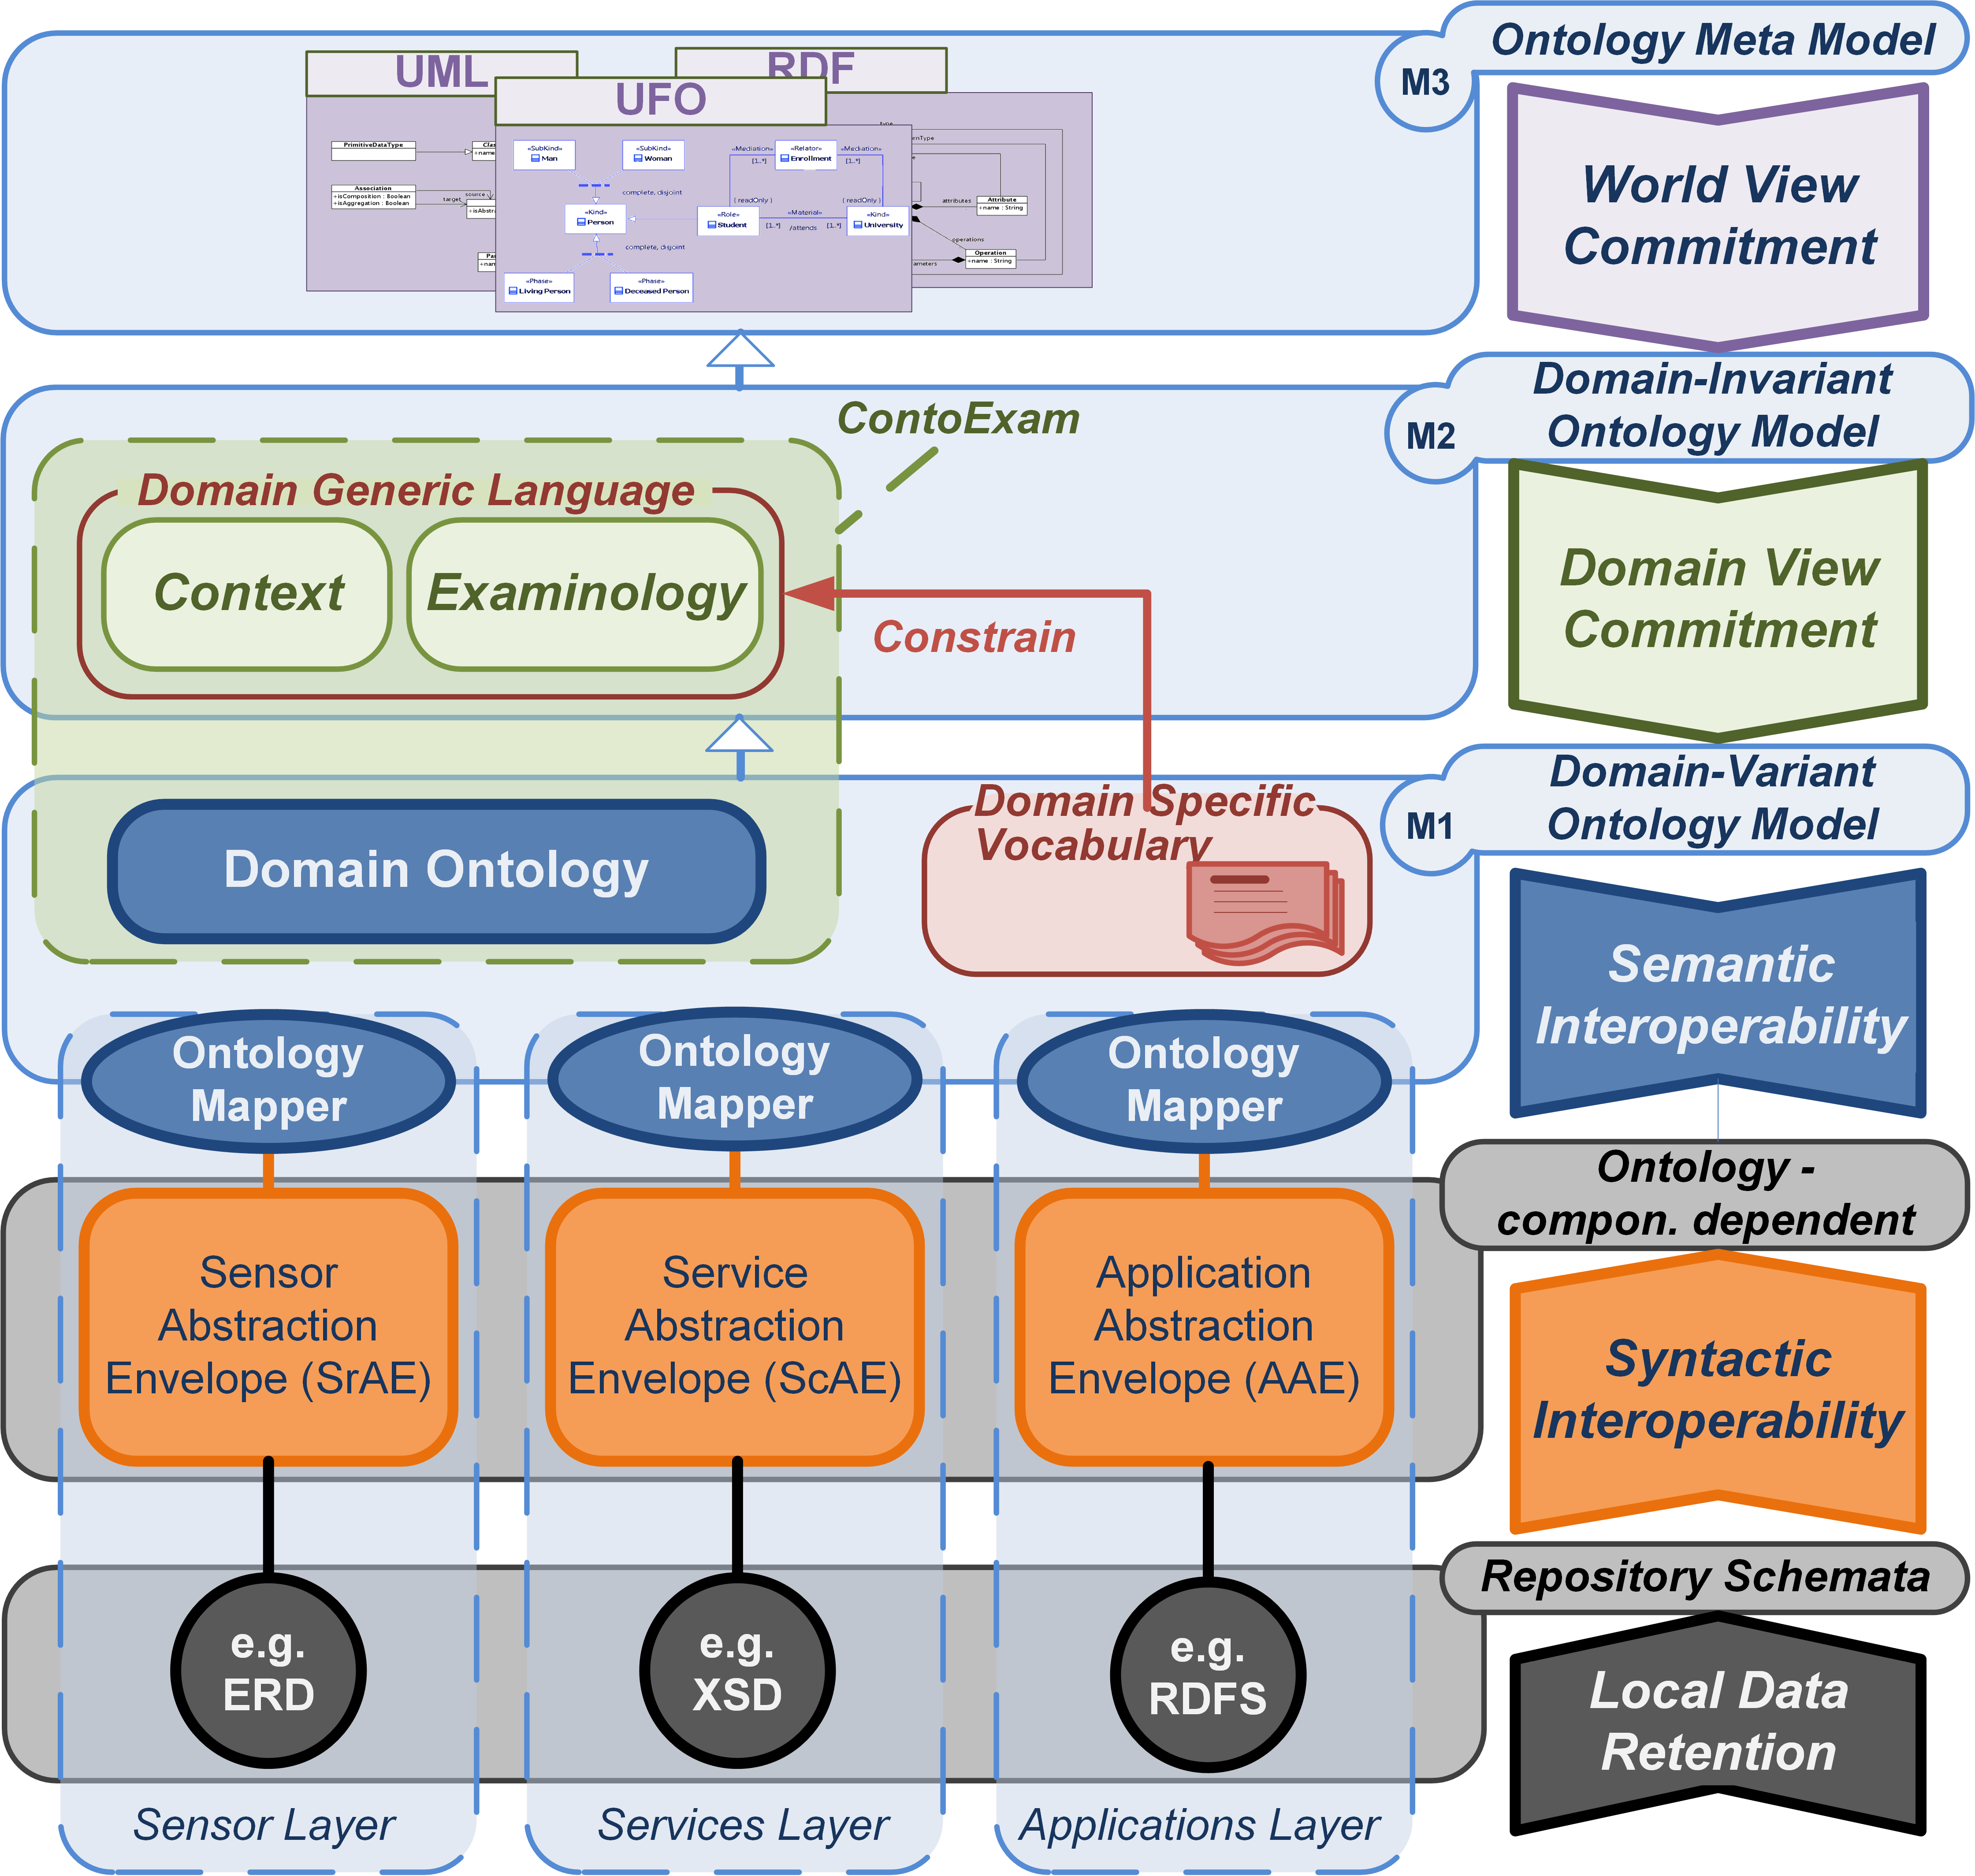
\includegraphics[width=4.66667in,height=4.4375in]{src/images/SemanticSoC.png}
\caption{An architecture for loosely coupled semantics, founded on
semantic SoC and semantic transparency (Brandt et al.
2013)}\label{fig:sSoC}
}
\end{figure}

\textbf{\emph{Achieve Scalable sIOP}}

Ensure that different semantic topologies remain possible:

\begin{enumerate}
\def\labelenumi{\roman{enumi}.}
\tightlist
\item
  Star alignments (central domain ontology, aligned to local ontologies)
  for relative stable and homogeneous domain semantics

  \begin{itemize}
  \tightlist
  \item
    Good: easy semantic governance
  \item
    Bad: very big semantic monolith, hence, low agility in dynamic
    environments
  \end{itemize}
\item
  Mesh alignments (bilateral alignments) for very dynamic and
  heterogeneous (domain) semantics, or low number of peers

  \begin{itemize}
  \tightlist
  \item
    Good: quickly established bilateral sIOP; granularity-on-demand,
    viz. intricate where necessary, coarse-grained where possible
  \item
    Bad: complicated semantic governance
  \end{itemize}
\item
  Mix-n-Match (coarse-grained star-alignment with specialised bilateral
  alignments) for the 70\% bulk * Good: controllable semantic
  governance; after central alignment, quickly established bilateral
  sIOP * Bad: slightly more complicated mediation due to double
  alignment support
\end{enumerate}

\hypertarget{iso42010-viewpoint-on-siop}{%
\chapter{ISO42010 viewpoint on sIOP}\label{iso42010-viewpoint-on-siop}}

Synopsis Consolidate the ideas on the bridgehead, spanning, roadway and
principles into an additional ISO42010 Architectural Viewpoint (sIOP)
that summarises all previous Sections as concerns on semantics and sIOP.
\textbf{\emph{Preferrably written by Eric.}}

\textbackslash{}end\{synopsis\}

\hypertarget{related-work}{%
\chapter{Related work}\label{related-work}}

Synopsis Group the papers into 3 (?) categories, and discuss their
strong and weak points in relation to sIOP and architecture in general,
and our paper specifically.

\textbackslash{}end\{synopsis\}

Text Discuss the following papers:

\begin{enumerate}
\def\labelenumi{\arabic{enumi}.}
\tightlist
\item
  M. B. Almeida, C. P. Pessanha, and R. Barcelos, ``Information
  Architecture for Organizations: An Ontological Approach,'' in Ontology
  in Information Science, C. Thomas, Ed. IntechOpen, 2018, pp.~1--27.
\item
  S. Yang, J. Guo, and R. Wei, ``Semantic interoperability with
  heterogeneous information systems on the internet through automatic
  tabular document exchange,'' Inf. Syst., vol.~69, pp.~195--217,
  Sep.~2017.
\item
  U. Aßmann, S. Zschaler, and G. Wagner, ``Ontologies, Meta-models, and
  the Model-Driven Paradigm,'' in Ontologies for Software Engineering
  and Software Technology, C. Calero, F. Ruiz, and M. Piattini, Eds.
  Springer-Verlag Berlin Heidelberg, 2006, pp.~249--273.
\item
  C. Atkinson and T. Kühne, ``The Essence of Multilevel Metamodeling,''
  LNCS, vol.~2185, pp.~19--33, 2001.
\item
  H. Carvalho e Silva, R. de Cassia Cordeiro de Castro, M. J. Negreiros
  Gomes, and A. Salles Garcia, Well-Founded IT Architecture Ontology: An
  Approach from a Service Continuity Perspective, vol.~294.
  Springer-Verlag Berlin Heidelberg, 2012.
\item
  R. Carraretto, ``Separating Ontological and Informational Concerns : A
  Model-driven Approach for Conceptual Modeling,'' Federal University of
  Espírito Santo, 2012.
\item
  C. L. B. Azevedo, M. E. Iacob, J. P. A. Almeida, M. J. van Sinderen,
  L. F. Pires, and G. Guizzardi, ``Modeling resources and capabilities
  in enterprise architecture: A well-founded ontology-based proposal for
  ArchiMate,'' Inf. Syst., vol.~54, pp.~235--262, 2015.
\item
  M. B. Almeida, C. P. Pessanha, and R. Barcelos, ``Information
  Architecture for Organizations: An Ontological Approach,'' in Ontology
  in Information Science, C. Thomas, Ed. IntechOpen, 2018, pp.~1--27.
\item
  D. Gasevic, D. Djuric, and V. Devedzic, Eds., Model Driven
  Architecture and Ontology Development. Springer Berlin Heidelberg New
  York, 2006. Particularly Part II: The Model Driven Architecture and
  Ontologies
\end{enumerate}

\hypertarget{discussion-future-work}{%
\chapter{Discussion \& future work}\label{discussion-future-work}}

Synopsis Address shortcomings that we discover throughout writing the
sections.

Conclude that by identifying a specific 42010 viewpoint on sIOP, a
necessary condition towards the preparation of a sIOP capability in a
software agent has been identified which can be applied to all MDE and
view-based software architectures.

\textbackslash{}end\{synopsis\}

\hypertarget{references--}{%
\chapter{References \{-\}}\label{references--}}

\setlength{\parindent}{-0.2in}

\setlength{\leftskip}{0.2in}

\setlength{\parskip}{8pt}

Note:{[} brandtp, 9/5/2018 Also show the ref-id per reference
\emph{duh}{]}

\hypertarget{refs}{}
\leavevmode\hypertarget{ref-Azevedo2015}{}%
Azevedo CL, Iacob ME, Almeida JPA, Sinderen MJ van, Pires LF, Guizzardi
G. 2015. Modeling resources and capabilities in enterprise architecture:
A well-founded ontology-based proposal for ArchiMate. Inf. Syst.
54:235--262;
doi:\href{https://doi.org/10.1016/j.is.2015.04.008}{10.1016/j.is.2015.04.008}.

\leavevmode\hypertarget{ref-Auxdfmann2006}{}%
Aßmann U, Zschaler S, Wagner G. 2006. Ontologies, Meta-models, and the
Model-Driven Paradigm. In \emph{Ontol. Softw. Eng. Softw. Technol.} (C.
Calero, F. Ruiz, and M. Piattinieds. ), pp. 249--273, Springer-Verlag
Berlin Heidelberg.

\leavevmode\hypertarget{ref-Brandt2018b}{}%
Brandt P, Basten T, Sinderen MJ van. 2018. Semantic mediation: from
alignment relations to data transcriptions. Prep.

\leavevmode\hypertarget{ref-Brandt2013}{}%
Brandt P, Basten T, Stuiik S. 2013. Semantic interoperability in sensor
applications making sense of sensor data. \ldots{} healthc. E- \ldots{}
5: 34--41.

\leavevmode\hypertarget{ref-Bricker2016}{}%
Bricker P. 2016. Ontological Commitment. In \emph{Stanford encycl.
Philos.} (E.N. Zaltaed. ),
\(\backslash\)url\{https://plato.stanford.edu/archives/win2016/entries/ontological-commitment/\};
Metaphysics Research Lab, Stanford University.

\leavevmode\hypertarget{ref-CarvalhoeSilva2012}{}%
Carvalho e Silva H, Cassia Cordeiro de Castro R de, Negreiros Gomes MJ,
Salles Garcia A. 2012. \emph{Well-Founded IT Architecture Ontology: An
Approach from a Service Continuity Perspective}. R. Benlamried..
Springer-Verlag Berlin Heidelberg.

\leavevmode\hypertarget{ref-Cregan2007}{}%
Cregan AM. 2007. Symbol grounding for the semantic web. W. Franconi, E
and Kifer, M and Mayed.. Semant. WEB res. Appl. Proc. 4519: 429--442.

\leavevmode\hypertarget{ref-Eco1976}{}%
Eco U. 1976. \emph{A theory of semiotics}. Indiana University Press /
London: Macmillam, Bloomington, IN.

\leavevmode\hypertarget{ref-Gamut1991}{}%
Gamut L. 1991. \emph{Logic, Language and Meaning, volume 1: Introduction
to Logic}. The University of Chicago Press.

\leavevmode\hypertarget{ref-Genesereth:1987dg}{}%
Genesereth MR, Nilsson NJ. 1987. \emph{Logical foundations of artificial
intelligence}. Morgan Kaufmann Publishers Inc.

\leavevmode\hypertarget{ref-Gonzalez-Perez2007}{}%
Gonzalez-Perez C, Henderson-Sellers B. 2007. Modelling software
development methodologies: A conceptual foundation. J. Syst. Softw.
80:1778--1796;
doi:\href{https://doi.org/10.1016/j.jss.2007.02.048}{10.1016/j.jss.2007.02.048}.

\leavevmode\hypertarget{ref-Greefhorst2011}{}%
Greefhorst D, Proper E. 2011. \emph{Architecture Principles, The
Cornerstones of Enterprise Architecture}. Springer Berlin Heidelberg.

\leavevmode\hypertarget{ref-Grice:1991BT}{}%
Grice HP. 1989. Logic and Conversation. In \emph{Stud. W. Words}, pp.
22--40, Harvard University Press, Cambridge, MA, USA.

\leavevmode\hypertarget{ref-Guarino1994b}{}%
Guarino N. 1994. The Ontological Level. R. Casati, B. Smith, and G.
Whiteeds. Philos. Cogn. Sci. Proc. 16th int. Wittgenstein symp.
443--456;
doi:\href{https://doi.org/10.1007/978-3-642-02463-4}{10.1007/978-3-642-02463-4}.

\leavevmode\hypertarget{ref-Guizzardi:2005vt}{}%
Guizzardi G. 2005. Ontological foundations for structural conceptual
models. PhD thesis, University of Twente, The Netherlands; CTIT,
Enschede, The Netherlands.

\leavevmode\hypertarget{ref-Guizzardi:2015ky}{}%
Guizzardi G, Wagner G, Almeida JPA, Guizzardi RSS. 2015. Towards
ontological foundations for conceptual modeling: The unified
foundational ontology (UFO) story. Appl. Ontol. 10:259--271;
doi:\href{https://doi.org/10.3233/AO-150157}{10.3233/AO-150157}.

\leavevmode\hypertarget{ref-Harnad1990}{}%
Harnad S. 1990. The Symbol Grounding Problem. Physica D 42. 335--346.

\leavevmode\hypertarget{ref-Henderson-Sellers2012}{}%
Henderson-Sellers B. 2012. \emph{On the mathematics of modelling,
metamodelling, ontologies and modelling languages}. Springer Berlin
Heidelberg, Berlin, Heidelberg.

\leavevmode\hypertarget{ref-Jansen2008}{}%
Jansen L. 2008. Categories : The Top-Level Ontology. In \emph{Appl.
Ontol. An introd.} (K. Munn and B. Smitheds. ), pp. 173--196, De
Gruyter.

\leavevmode\hypertarget{ref-Kuhn2009}{}%
Kuhn W. 2009. Semantic engineering. In \emph{Res. Trends geogr. Inf.
Sci. Lect. Notes geoinf. Cartogr.} (G. Navratiled. ), pp. 63--76,
Springer Berlin Heidelberg.

\leavevmode\hypertarget{ref-Ogden1989}{}%
Ogden CK, Richards IA. 1989. \emph{The Meaning of Meaning: A Study of
the Influence of Language upon Thought and of the Science of Symbolism}.
with a pre. Harcourt Brace Jovanovich, New York, USA.

\leavevmode\hypertarget{ref-Quine:1953er}{}%
Quine WVO. 1961. From a logical point of view. Br. Dent. J. 195: 229.

\leavevmode\hypertarget{ref-Searle:1980hw}{}%
Searle JR. 1980. Minds, brains, and programs. Behav. Brain Sci. 3:
417--424.

\leavevmode\hypertarget{ref-Smith2005}{}%
Smith B. 2005. Against fantology. In \emph{Exp. Anal.} (M. Reicher and
J. Marekeds. ), pp. 153--170, HPT\&ÖPV, Vienna.

\leavevmode\hypertarget{ref-Sowa:2000di}{}%
Sowa JF. 2000. Ontology, metadata, and semiotics. Lect. Notes Comput.
Sci. (including Subser. Lect. Notes Artif. Intell. Lect. Notes
Bioinformatics) 1867:55--81;
doi:\href{https://doi.org/10.1007/10722280_5}{10.1007/10722280\_5}.

\leavevmode\hypertarget{ref-Steels:2008tr}{}%
Steels L. 2012. The symbol grounding problem has been solved, so what's
next. In \emph{Symb. Embodiment debates mean. Cogn.} (M. de Vega, A.
Glenberg, and A. Graessereds. ), pp. 223--244, Oxford University Press,
Oxford, UK.

\leavevmode\hypertarget{ref-XiuquanLi2017}{}%
Xiuquan Li, Tao Zhang. 2017. An exploration on artificial intelligence
application: From security, privacy and ethic perspective. J. Zhu, E.-B.
Lin, and T. Lieds. 2017 ieee 2nd int. Conf. Cloud comput. Big data anal.
416--420;
doi:\href{https://doi.org/10.1109/ICCCBDA.2017.7951949}{10.1109/ICCCBDA.2017.7951949}.

%\chapter*{References}
% --- index --- --- --- --- ---


\printindex

%ACKNOWLEDGMENTS are optional
%\chapter*{Acknowledgments}
% % 
\end{document}
